\documentclass[twoside,11pt]{article}\usepackage[]{graphicx}\usepackage[]{xcolor}
% maxwidth is the original width if it is less than linewidth
% otherwise use linewidth (to make sure the graphics do not exceed the margin)
\makeatletter
\def\maxwidth{ %
  \ifdim\Gin@nat@width>\linewidth
    \linewidth
  \else
    \Gin@nat@width
  \fi
}
\makeatother

\definecolor{fgcolor}{rgb}{0.345, 0.345, 0.345}
\newcommand{\hlnum}[1]{\textcolor[rgb]{0.686,0.059,0.569}{#1}}%
\newcommand{\hlstr}[1]{\textcolor[rgb]{0.192,0.494,0.8}{#1}}%
\newcommand{\hlcom}[1]{\textcolor[rgb]{0.678,0.584,0.686}{\textit{#1}}}%
\newcommand{\hlopt}[1]{\textcolor[rgb]{0,0,0}{#1}}%
\newcommand{\hlstd}[1]{\textcolor[rgb]{0.345,0.345,0.345}{#1}}%
\newcommand{\hlkwa}[1]{\textcolor[rgb]{0.161,0.373,0.58}{\textbf{#1}}}%
\newcommand{\hlkwb}[1]{\textcolor[rgb]{0.69,0.353,0.396}{#1}}%
\newcommand{\hlkwc}[1]{\textcolor[rgb]{0.333,0.667,0.333}{#1}}%
\newcommand{\hlkwd}[1]{\textcolor[rgb]{0.737,0.353,0.396}{\textbf{#1}}}%
\let\hlipl\hlkwb

\usepackage{framed}
\makeatletter
\newenvironment{kframe}{%
 \def\at@end@of@kframe{}%
 \ifinner\ifhmode%
  \def\at@end@of@kframe{\end{minipage}}%
  \begin{minipage}{\columnwidth}%
 \fi\fi%
 \def\FrameCommand##1{\hskip\@totalleftmargin \hskip-\fboxsep
 \colorbox{shadecolor}{##1}\hskip-\fboxsep
     % There is no \\@totalrightmargin, so:
     \hskip-\linewidth \hskip-\@totalleftmargin \hskip\columnwidth}%
 \MakeFramed {\advance\hsize-\width
   \@totalleftmargin\z@ \linewidth\hsize
   \@setminipage}}%
 {\par\unskip\endMakeFramed%
 \at@end@of@kframe}
\makeatother

\definecolor{shadecolor}{rgb}{.97, .97, .97}
\definecolor{messagecolor}{rgb}{0, 0, 0}
\definecolor{warningcolor}{rgb}{1, 0, 1}
\definecolor{errorcolor}{rgb}{1, 0, 0}
\newenvironment{knitrout}{}{} % an empty environment to be redefined in TeX

\usepackage{alltt}

% Any additional packages needed should be included after jmlr2e.
% Note that jmlr2e.sty includes epsfig, amssymb, natbib and graphicx,
% and defines many common macros, such as 'proof' and 'example'.
%
% It also sets the bibliographystyle to plainnat; for more information on
% natbib citation styles, see the natbib documentation, a copy of which
% is archived at http://www.jmlr.org/format/natbib.pdf

% Available options for package jmlr2e are:
%
%   - abbrvbib : use abbrvnat for the bibliography style
%   - nohyperref : do not load the hyperref package
%   - preprint : remove JMLR specific information from the template,
%         useful for example for posting to preprint servers.
%
% Example of using the package with custom options:
%
% \usepackage[abbrvbib, preprint]{jmlr2e}

\usepackage{jmlr2e}
% extra packages
\usepackage{longtable}
\usepackage{colortbl}
\usepackage{amsmath}
\usepackage{booktabs}
\usepackage{caption}
\usepackage{multirow}
\usepackage{hyperref}
\hypersetup{hidelinks}
\usepackage{geometry}
\usepackage{pdflscape}
\usepackage{bm}
\usepackage{algorithm, algcompatible, algpseudocode}
\usepackage{eqparbox}

\DeclareMathOperator*{\argmin}{argmin}
\DeclareMathOperator*{\argmax}{argmax}

\newdimen{\algindent}
\setlength\algindent{1.5em}          % algorithmic indent=1.5em
\algnewcommand\LeftComment[2]{%
\hspace{#1\algindent}$\triangleright$ \eqparbox{COMMENT}{#2} \hfill %
}

\algnewcommand{\algorithmicgoto}{\textbf{go to}}%
\algnewcommand{\Goto}[1]{\algorithmicgoto~\ref{#1}}%

\DeclareCaptionLabelFormat{AppendixTables}{A.#2}

\definecolor{lightgray}{rgb}{0.83, 0.83, 0.83}

% Definitions of handy macros can go here

\newcommand{\dataset}{{\cal D}}
\newcommand{\fracpartial}[2]{\frac{\partial #1}{\partial  #2}}
\newcommand{\ie}{that is}
\newcommand{\eg}{for example}
\newcommand{\cstat}{\widehat{\text{C}}(t)}
\newcommand{\bstat}{\widehat{\text{BS}}(t)}
\newcommand{\bsbar}{\mathcal{\widehat{BS}}(t_1, t_2)}
\newcommand{\bskap}{\mathcal{\widehat{BS}}_0(t_1, t_2)}

\newcommand{\ntrain}{N_{\text{train}}}
\newcommand{\ntest}{N_{\text{test}}}

\newcommand{\secref}[1]{Section \ref{#1}}

\newcommand{\tabref}[1]{Table \ref{#1}}
\newcommand{\tabrefAppendix}[1]{Table A.\ref{#1}}

% Heading arguments are {volume}{year}{pages}{date submitted}{date published}{paper id}{author-full-names}

\jmlrheading{1}{2000}{1-48}{4/00}{10/00}{meila00a}{Marina Meil\u{a} and Michael I. Jordan}

% Short headings should be running head and authors last names

\ShortHeadings{Accelerated oblique random survival forests}{Jaeger et al}
\firstpageno{1}
\IfFileExists{upquote.sty}{\usepackage{upquote}}{}
\begin{document}

\title{Accelerated oblique random survival forests}

\author{\name Byron C. Jaeger \email bjaeger@wakehealth.edu \\
       \addr Department of Biostatistics and Data Science\\
       Wake Forest University School of Medicine\\
       Winston-Salem, NC 27157, USA
       \AND
       \name Sawyer Welden \email swelden@wakehealth.edu \\
       \addr Department of Biostatistics and Data Science\\
       Wake Forest University School of Medicine\\
       Winston-Salem, NC 27157, USA
       \AND
       \name Kristin Lenoir \email klenoir@wakehealth.edu \\
       \addr Department of Biostatistics and Data Science\\
       Wake Forest University School of Medicine\\
       Winston-Salem, NC 27157, USA
       \AND
       \name Jaime L Speiser \email jspeiser@wakehealth.edu \\
       \addr Department of Biostatistics and Data Science\\
       Wake Forest University School of Medicine\\
       Winston-Salem, NC 27157, USA
       \AND
       \name Matthew Segar \email Matthew.Segar@UTSouthwestern.edu \\
       \addr Division of Cardiology, Department of Internal Medicine, \\
       University of Texas Southwestern Medical Center, Dallas
       \AND
       \name Nicholas M. Pajewski \email npajewsk@wakehealth.edu \\
       \addr Department of Biostatistics and Data Science\\
       Wake Forest University School of Medicine\\
       Winston-Salem, NC 27157, USA}

\editor{TBD}

\maketitle



\newpage

\begin{abstract}%   <- trailing '%' for backward compatibility of .sty file

The oblique random survival forest (RSF) is an ensemble supervised learning method for right-censored outcomes. Trees in the oblique RSF are grown using linear combinations of predictors to create branches, whereas in the standard RSF a single predictor is used. Oblique RSF ensembles often have higher prediction accuracy than standard RSF ensembles, but the additional computational overhead of finding an optimal combination of predictors is a severe limitation. In addition, few methods have been developed for interpretation of oblique RSF ensembles. We introduce and evaluate a method to increase computational efficiency of the oblique RSF and a method to estimate importance of individual predictor variables with the oblique RSF. Our strategy to reduce computational overhead makes use of Newton-Raphson scoring, a classical optimization technique that we apply to the Cox partial likelihood function. We estimate importance of predictors for the oblique RSF by negating each coefficient used for the given predictor in linear combinations, and then computing the reduction in out-of-bag accuracy. In numeric experiments, we find that our implementation of the oblique RSF is roughly 500 times faster with equivalent or superior prediction accuracy compared to existing software to fit oblique RSFs. We find in simulation studies that `negation importance' discriminates between signal and noise predictors more reliably than permutation importance, Shapley additive explanations, and a previously introduced technique to measure variable importance with oblique RSFs based on analysis of variance. All methods pertaining to oblique RSFs in the current study are available in the \texttt{aorsf} R package.

\end{abstract}

\begin{keywords}
  Random Forests, Survival, Efficient, Variable Importance
\end{keywords}

\section{Introduction}

The random survival forest (RSF; \citet{ishwaran2008random, hothorn2006unbiased}) is a supervised learning algorithm that can be used for risk prediction \citep{wang2017selective}, which may reduce the burden of disease by guiding strategies for prevention and treatment in a wide range of medical domains \citep{moons2012riskII, moons2012riskI}. Similar to random forests (RFs) for classification and regression \citep{breiman2001random}, The RSF is a large set of de-correlated and randomized decision trees, with each tree contributing to the ensemble's prediction function. Notable characteristics of the RSF include uniform convergence of its ensemble survival prediction function to the true survival function, first shown by \citet{ishwaran2010consistency} and later by \citet{cui2017consistency} under more general conditions. However, \citet{cui2017consistency} noted that the RSF is at a disadvantage when predictors are correlated and some are not relevant to the censored outcome, which is a strong possibility when large medical databases are leveraged for risk prediction.

A potential approach to improve the RSF when predictors are correlated and some are not relevant to the censored outcome is to use oblique decision trees instead of axis based trees. Axis based trees split data using a single predictor, creating decision boundaries that are perpendicular or parallel to axes of the predictor space \citep[see][Chapter~2]{breiman2017classification}. Oblique trees split data using a linear combination of predictors, creating decision boundaries that are neither parallel nor perpendicular to axes of their contributing predictors \citep[see][Chapter~5]{breiman2017classification}. \citet{menze2011oblique} examined prediction accuracy of RFs in the presence of correlated predictors and found that oblique RFs had substantially higher prediction accuracy compared to axis-based RFs. Similarly, \citet{jaeger2019oblique} found that growing RSFs with oblique rather than axis-based survival trees reduced the RSF's concordance error, with improvements ranging from 2.5\% to 24.9\% depending on the data analyzed.

Oblique trees have at least two notable drawbacks compared to axis-based trees. First, finding a locally optimal oblique decision rule may require exponentially more computation than an axis-based rule. If $p$ predictors are potentially used to split $n$ observations, up to $\mathcal{O}(n^p)$ oblique splits can be assessed versus $\mathcal{O}(n \cdot p)$ axis-based splits \citep{heath1993induction, murthy1994system}. Second, estimating variable importance (VI) using permutation (a standard method for RFs) may be less effective in ensembles of oblique trees, as permuting the values of one predictor may not destabilize decisions that are based on many predictors. Although VI is one of the most widely used strategies to interpret random forests \citep{ishwaran2019standard}, few studies have investigated VI for oblique random forests \citep[see][Section~5]{menze2011oblique}, and fewer have investigated VI specifically for the oblique RSF.

This study makes two contributions to oblique RSFs. First, we reduce their computational cost (\ie, accelerate them) with a scalable algorithm to identify linear combinations of coefficients. In a general benchmark experiment including 31 risk prediction tasks, we show that accelerated oblique RSFs are roughly 500 times faster with equivalent or superior prediction accuracy compared to existing routines to fit oblique RSFs. Second, we improve their interpretability with `negation VI', a method to estimate VI that engages with coefficients in linear combinations of predictors instead of permuting predictor values. In simulation studies where VI is estimate using permutation, analysis of variance (ANOVA; see \citet{menze2011oblique}), and approximations of Shapley values, we find that negation VI improves the oblique RSF's ability to discriminate between correlated signal and noise variables. The accelerated oblique RSF and multiple methods to compute VI for oblique RSFs (permutation, ANOVA, and negation) are available in the \texttt{aorsf} R Package.


% However, there remains considerable potential to improve the RSF in settings where training samples are not large enough to guarantee asymptotic properties or do not align with the conditions required for consistency of the RSF.


% Random forests (RFs) are large sets of de-correlated, randomized decision trees \citep{breiman2001random}, which can be axis based or oblique.Although using oblique rather than axis-based trees to grow a RSF may improve its prediction accuracy,


\section{Related work}

\subsection{Axis-based and oblique random forests}

After \citet{breiman2001random} introduced the axis-based and oblique RF, numerous methods were developed to grow oblique RFs for classification or regression tasks \citep{menze2011oblique, zhang2014oblique, rainforth2015canonical, zhu2015reinforcement, poona2016investigating, qiu2017oblique, tomita2020sparse, katuwal2020heterogeneous}. However, oblique splitting approaches for classification or regression may not generalize to survival \citep[\eg, see][Section~4.5.1]{zhu2013tree}, and most research involving the RSF has focused on forests with axis-based trees \citep{wang2017selective}.

Building on prior research for bagging survival trees \citep{hothorn2004bagging}, \citet{hothorn2006unbiased} developed an axis-based RSF in their framework for unbiased recursive partitioning, more commonly referred to as the conditional inference forest (CIF). \citet{zhou2016random} developed a rotation forest based on the CIF and \citet{wang2017random} developed a method for extending the predictor space of the CIF. \citet{ishwaran2008random} developed an axis-based RSF with strict adherence to the rules for growing trees proposed in \citet{breiman2001random}. \citet{jaeger2019oblique} developed the oblique RSF following the bootstrapping approach described in Breiman's original RF and incorporating early stopping rules from the CIF.

\subsection{Variable importance}

\citet{breiman2001random} introduced permutation VI, defined for each predictor as the difference in a RF's estimated generalization error before versus after the predictor's values are randomly permuted. \citet{strobl2007bias} identified bias in permutation VI driven by variable selection bias and effects induced by bootstrap sampling, and proposed an unbiased permutation VI based on unbiased recursive partitioning (see \citet{hothorn2006unbiased}). \citet{menze2011oblique} introduced an approach to estimate VI for oblique RFs that computes an analysis of variance (ANOVA) table in non-leaf nodes to obtain p-values for each predictor contributing to the node. The ANOVA VI\footnote{\citet{menze2011oblique} name their method `oblique RF VI', but we use the name `ANOVA VI' in this article to avoid confusing Menze's approach with other approaches to estimate VI for oblique RFs.} is then defined for each predictor as the number of times a p-value associated with the predictor is $\leq 0.01$ while growing a forest. \citet{lundberg2017unified} introduced a method to estimate VI using SHapley Additive exPlanation (SHAP) values, which estimate the contribution of a predictor to a model's prediction for a given observation. SHAP VI is computed for each predictor by taking the mean absolute value of SHAP values for that predictor across all observations in a given set.

% Several supervised learning algorithms can develop prediction functions for right-censored time-to-event outcomes, henceforth referred to as survival outcomes. \cite{ishwaran2008random} developed the RF for survival, an extension of the RF for regression and classification developed by \citet{breiman2001random}. Fast algorithms to fit the RF for survival are available in the \texttt{randomForestSRC} R package \citep{randomForestSRC}. A similar implementation of the RF for survival can be found in the \texttt{ranger} R package \citep{ranger}, which is particularly suited for high dimensional data. The RF for survival can also be fit using unbiased recursive partitioning \citep{cif} via the \texttt{party} R package \citep{hothorn2010party}.

\section{The acceleracted oblique random survival forest}

Consider the usual framework for survival analysis with training data $$\dataset_{\text{train}} = \left\{ (T_i, \delta_i, \bm{x}_{i}) \right\}_{i=1}^{N_{\text{train}}}.$$ Here, $T_i$ is the event time if $\delta_i=1$ and last point of contact if $\delta_i=0$, and $\bm{x}_i$ is a vector of predictors values. Assuming there are no ties, let $t_1 < \, \ldots \, < t_m$ denote the $m$ unique event times in $\dataset_{\text{train}}$.

To accelerate the oblique RSF, we propose to identify linear combinations of predictor variables in non-leaf nodes by applying Newton Raphson scoring to the partial likelihood function of the Cox regression model:
\begin{equation}\label{eqn:cox-partial-likelihood}
L(\bm\beta) = \prod_{i=1}^m \frac{e^{\bm{x}_{j(i)}^T \bm\beta}}{\sum_{j \in R_i} e^{\bm{x}_j^T \bm\beta}},
\end{equation}
where $R_i$ is the set of indices, $j$, with $T_j \geq t_i$ (i.e., those still at risk at time $t_i$), and $j(i)$ is the index of the observation for which an event occurred at time $t_i$. Newton Raphson scoring is an extremely fast estimation procedure, and the \texttt{survival} package includes documentation that outlines how to efficiently program it \citep{therneau_survival_2022}. Briefly, a vector of estimated regression coefficients, $\hat{\beta}$, is updated in each step of the procedure based on its first derivative, $U(\hat{\beta})$, and second derivative, $H(\hat{\beta})$:
$$ \hat{\beta}^{k+1} =  \hat{\beta}^{k} + U(\hat{\beta} = \hat{\beta}^{k})\, H^{-1}(\hat{\beta} = \hat{\beta}^{k}) $$

For statistical inference, it is recommended to complete iterations of Newton Raphson scoring until a convergence threshold is met. However, to identify a valid linear combination of predictors, only one iteration of Newton Raphson scoring is needed. In \secref{sec:results_pred}, we formally test whether growing oblique survival trees using one iteration of Newton Raphson scoring is sufficient (\ie, provides equivalent prediction accuracy) compared to iterating until a convergence threshold is met.

Algorithm \ref{alg:aorsf} presents our approach to fitting an oblique survival tree in the accelerated oblique RSF using default values from the \texttt{aorsf} R package. Several steps are taken to reduce computational overhead. First, memory is conserved by conducting bootstrap resampling via randomly generated bootstrap weights. Weights are integer valued, with a weight of $v$ indicating an observation was sampled $v$ times. Second, early stopping is applied to the tree growing procedure if a statistical criterion is not met. In our case, the criterion is based on the magnitude of a log-rank test statistic corresponding to splitting the data at a current node. Third, instead of greedy recursive partitioning, we use a `good enough' approach. More specifically, instead of computing a log-rank test statistic for several different linear combinations of variables and proceeding with the highest scoring option, we identify an optimal cut-point for one linear combination of variables and assess whether using this combination will create a split that passes the criterion for splitting a node. If it does not pass the criterion, then another linear combination will be tested, with the maximum number of attempts set by the parameter \texttt{n\_retry}. Often a `good-enough` split can be found in just one attempt when the training set is large, which gives the accelerated oblique RSF a computational advantage in larger training sets compared to greedy partitioning.

\begin{algorithm}
    \caption{Accelerated oblique random survival tree using default parameters.} \label{alg:aorsf}
  \begin{algorithmic}[1]
    \Require Training data $\dataset_{\text{train}} = \left\{ (T_i, \delta_i, \bm{x}_{i}) \right\}_{i=1}^{N_{\text{train}}}$, $\text{mtry} = \sqrt{\text{ncol}(\bm{x}_{\text{train}})}$, $\text{n\_split} = 5$, $\text{n\_retry} = 3$, and $\text{split\_min\_stat} = 3.841459$
    \State $\mathcal{T} \gets \emptyset$
    \State $w \gets \text{sample}(\text{from} = \left\{0, \ldots, 10\right\},\,\text{size} = \text{nrow}(\bm{x}_{\text{train}}),\, \text{replace} = \text{T})$
    \State $\dataset_{\text{in-bag}} \gets \text{subset}(\dataset_{\text{train}},\,\text{rows} = \text{which}(w > 0))$
    \State $w \gets \text{subset}(w,\, \text{which}(w > 0))$
    \State $\text{node\_assignments} \gets \text{rep}(1,\,\text{times} = \text{nrow}(\bm{x}_{\text{in-bag}}))$
    \State $\text{nodes\_to\_split} \gets \{1\}$
     \Repeat
     \For{$\text{node} \in \text{nodes\_to\_split}$}
       \State $\text{n\_try} \gets 1$
       \State $\text{node\_rows} \gets \text{which}(\text{node\_assignments} \equiv \text{node})$
       \State $\text{node\_cols} \gets \text{sample}(\text{from} = \left\{1, \ldots, \text{ncol}(\bm{x})\right\},\, \text{size} = \text{mtry},\,\text{replace} = \text{F})$ \label{marker}
       \State $\dataset_{\text{node}} \gets \text{subset}(\dataset_{\text{in-bag}},\,\text{rows} = \text{node\_rows},\,\text{columns} = \text{node\_cols})$
       \State $\beta \gets \text{newt\_raph}(\dataset_{\text{node}},\, \text{weights} = \text{subset}(w, \text{node\_rows}),\, \text{max\_iter} = 1)$
       \State $\eta \gets \bm{x}_{\text{node}} \times \beta$
       \State $\mathcal{C} \gets \text{sample}(\text{from} = \text{unique}(\eta),\, \text{size} = \text{n\_split},\,\text{replace} = \text{F})$
       \State $c \gets \argmax_{c^* \in \mathcal{C}} \left\{ \text{log\_rank\_stat}(\eta, c^*) \right\}$
       \If{$\text{log\_rank\_stat}(\eta, c) \geq \text{split\_min\_stat}$}
         \State $\mathcal{T} \gets \text{add\_node}(\mathcal{T},\, \text{name} = \text{node},\, \text{beta} = \beta,\, \text{cutpoint} = c)$
         \State \LeftComment{0}{Right node logic omitted for brevity (identical to left node logic)}
         \State $\text{node\_left\_name} \gets \text{max}(\text{node\_assignments}) + 1$
         \State $\text{node\_left\_rows} \gets \text{subset}(\text{node\_rows},\,\text{which}(\eta \leq c))$
         \State $\text{subset}(\text{node\_assignments}, \text{node\_left\_rows}) \gets \text{node\_left\_name}$
         \If{$\text{is\_splittable}(\text{subset}(\text{node\_assignments}, \text{node\_left\_rows}))$}
           \State $\text{nodes\_to\_split} \gets \text{nodes\_to\_split} \cup \text{node\_left\_name}$
         \Else
           \State $\mathcal{T} \gets \text{add\_leaf}(\mathcal{T},\, \text{data} = \text{subset}(\dataset_{\text{node}},\,\text{rows} = \text{node\_left\_rows}))$
         \EndIf
       \ElsIf{$\text{n\_try} \leq \text{n\_retry}$}
         \State $\text{n\_try} \gets \text{n\_try} + 1$
         \State \Goto{marker}
       \Else
         \State $\mathcal{T} \gets \text{add\_leaf}(\mathcal{T},\, \text{data} =\dataset_{\text{node}})$
       \EndIf
       \State $\text{nodes\_to\_split} \gets \text{nodes\_to\_split} \setminus \text{node}$
     \EndFor
  \Until{$\text{nodes\_to\_split} = \emptyset$}
  \State \Return $\mathcal{T}$
  \end{algorithmic}
\end{algorithm}

\subsection{Negation variable importance}

Negation VI is similar to permutation VI in that it measures how much a model’s prediction error increases when a variable’s role in the model is de-stabilized. More specifically, negation VI measures the increase in an oblique RF's prediction error after flipping the sign of all coefficients linked to a variable (\ie, negating them). As the magnitude of a coefficient increases, so does the probability that negating it will change the oblique RF's predictions. For the current study, we use Harrell's concordance (C)-statistic \citep{harrell1982evaluating} to measure change in prediction error when computing negation VI.

Negation VI has several characteristics that may be helpful. First, although the current article focuses on oblique RSFs and uses Harrell's C-statistic, negation VI can be applied to any oblique RF using any valid error function.\footnote{The \texttt{aorsf} package enables customized functions to be applied in lieu of the default C-statistic (see \texttt{?aorsf::orsf\_vi\_negate})}. Second, since the coefficients in each non-leaf node of an oblique tree are adjusted for the accompanying predictors, negation VI may provide better estimation of VI in the presence of correlated variables compared to standard VI techniques. This conjecture is formally assessed in \secref{sec:results_vi}. Third, unlike permutation importance, negation VI is non-random and hence reproducible without setting a random seed. Along these lines, since negation VI does not permute variables, the analyst need not worry about impossible combinations of predictors that may occur when one predictor is randomly permuted, such as having a negative status for type 2 diabetes and having Hemoglobin A1c level $\geq$ 6.5\% as a result of randomly permuting the values of Hemoglobin A1c.

\section{Numeric experiments}

\subsection{Benchmark of prediction accuracy and computational efficiency} \label{sec:bm_pred}

The aim of this numeric experiment is to evaluate and compare the accelerated oblique RSF with its predecessor (the oblique RSF from the \texttt{obliqueRSF} R package) and with other machine learning algorithms for risk prediction. Inferences drawn from this experiment include equivalence and inferiority tests based on Bayesian linear mixed models.

\subsubsection{Learners} \label{sec:learners}

We consider four classes of learners: RSFs (both axis based and oblique), boosting ensembles, regression models, and neural networks (\tabref{tab:learners}). For each class, we synchronized shared tuning parameters. For example, for RSF learners, we set the minimum node size (a parameter shared by all RSF learners) as 10. Additionally, for RSF learners, the number of randomly selected predictors was the square root of the total number of predictors rounded to the nearest integer, and the number of trees in the ensemble was 500. For boosting, regression, and neural network learners, nested 10-fold cross-validation was applied to tune relevant model parameters. Specifically, tuning for boosting models included identifying the number of steps to complete. For regression models, tuning was used to identify the magnitude of penalization. For neural networks, the number and density of layers was tuned.

\newgeometry{margin=1cm} % modify this if you need even more space
\begin{landscape}

\begin{table}[h!]
\centering
\begin{tabular}{p{2cm} | p{3cm} p{4cm} p{12cm}}
 \hline
 Learner Class & Software & Learners & Description \\ [0.5ex]
 \hline\hline
 \multicolumn{3}{l}{\textit{Random Survival Forests}}\\
 \hline\hline

 Axis based &

 \href{https://www.randomforestsrc.org/index.html}{\texttt{RandomForestSRC}} \newline
 \href{https://CRAN.R-project.org/package=ranger}{\texttt{ranger}} \newline
 \href{http://party.r-forge.r-project.org/}{\texttt{party}} \newline
 \href{https://github.com/whcsu/rotsf}{\texttt{rotsf}} \newline
 \href{https://github.com/whcsu/rsfse}{\texttt{rsfse}} &

 \texttt{rsf-standard} \newline
 \texttt{rsf-extratrees} \newline
 \texttt{cif-standard} \newline
 \texttt{cif-rotate} \newline
 \texttt{cif-spacextend} &

 \texttt{rsf-standard} grows survival trees following Leo Breiman's original random forest algorithm with variables and cut-points selected to maximize a log-rank statistic. \texttt{rsf-extratrees} grows survival trees with randomly selected features and cut-points. \texttt{cif-standard} uses the framework of conditional inference to grow survival trees. \texttt{cif-rotate} extends \texttt{cif-standard} by applying principal component analysis to random subsets of data prior to growing each survival tree. \texttt{cif-spacextend} derives new predictors for each tree in the ensemble, separately. \\ \hline


 Oblique &


 \href{https://CRAN.R-project.org/package=obliqueRSF}{\texttt{obliqueRSF}} \newline
 \href{https://bcjaeger.github.io/aorsf/}{\texttt{aorsf}} &

 \texttt{obliqueRSF-net} \newline
 \texttt{aorsf-net} \newline
 \texttt{aorsf-fast} \newline
 \texttt{aorsf-cph} \newline
 \texttt{aorsf-extratrees} &


 Oblique survival trees following Leo Breiman's random forest algorithm. Linear combinations of inputs are derived using \texttt{glmnet} in \texttt{obliqueRSF-net} and \texttt{aorsf-net}, using Newton Raphson scoring for the Cox partial likelihood function in \texttt{aorsf-fast} (1 iteration of scoring) and \texttt{aorsf-cph} (up to 20 iterations), and chosen randomly from a uniform distribution in \texttt{aorsf-extratrees}. Cut-points are selected from 5 randomly selected candidates to maximize a log-rank statistic. \\

 \hline\hline
 \multicolumn{3}{l}{\textit{Boosting ensembles}}\\
 \hline\hline

 Trees &

 \href{https://xgboost.readthedocs.io/en/stable/#}{\texttt{xgboost}} &

 \texttt{xgboost-cox} \newline
 \texttt{xgboost-aft} &

 \texttt{xgboost-cox} maximizes the Cox partial likelihood function, whereas \texttt{xgboost-aft} maximizes the accelerated failure time likelihood function. Nested cross validation (5 folds) is applied to tune the number of trees grown, the minimum number of observations in a leaf node was 10, the maximum depth of trees was 6, and $\sqrt{p}$ variables were considered randomly for each tree split, where $p$ is the total number of predictors. \\

 \hline\hline
 \multicolumn{3}{l}{\textit{Regression models}}\\
 \hline\hline

 Cox Net &

 \texttt{glmnet} &

 \texttt{glmnet-cox} &

 The Cox proportional hazards model is fit using an elastic net penalty. Nested cross validation (5 folds) is applied to tune penalty terms.\\

 \hline\hline
 \multicolumn{3}{l}{\textit{Neural networks}}\\
 \hline\hline

 Cox Time &

 \href{https://raphaels1.github.io/survivalmodels/}{\texttt{survivalmodels}} &

 \texttt{nn-cox} &

 A neural network based on the proportional hazards model with time-varying effects. Nested cross-validation was applied to select the number of layers (from 1 to 8), the number of nodes in each layer (from $\sqrt{p}$/2 to $\sqrt{p}$), and the number of epochs to complete (up to 500). A drop-out rate of 10\% was applied during training.   \\
 \hline

\end{tabular}
\caption{Learning algorithms assessed in numeric studies}
\label{tab:learners}
\end{table}

\end{landscape}
\restoregeometry



\subsubsection{Evaluation of prediction accuracy} \label{sec:prediction_accuracy}

Our primary metric for evaluating the accuracy of predicted risk is the integrated and scaled Brier score \citep{graf1999assessment}. Consider a testing data set:
$$\dataset_{\text{test}} = \left\{ (T_i, \delta_i, x_{i}) \right\}_{i=1}^{N_{\text{test}}}.$$
Let $\widehat{S}(t \mid x_i)$ be the predicted probability of survival up to a given prediction horizon of $t > 0$.
 For observation $i$ in $\dataset_{\text{test}}$, let $\widehat{S}(t \mid \bm{x}_i)$ be the predicted probability of survival up to a given prediction horizon of $t > 0$. Define \begin{align*}
\bstat = \frac{1}{\ntest} \sum_{i=1}^{\ntest} &\{ \widehat{S}(t \mid \bm{x}_i)^2 \cdot I(T_i \leq t, \delta_i = 1) \cdot \widehat{G}(T_i)^{-1} \\ &+ [1-\widehat{S}(t \mid \bm{x}_i)]^2 \cdot I(T_i > t) \cdot \widehat{G}(t)^{-1}\}
\end{align*} where $\widehat{G}(t)$ is the Kaplan-Meier estimate of the censoring distribution. As $\bstat$ is time dependent, integration over time provides a summary measure of performance over a range of plausible prediction horizons. The integrated $\bstat$ is defined as \begin{equation}
\bsbar = \frac{1}{t_2 - t_1}\int_{t_1}^{t_2} \widehat{\text{BS}}(t) dt.
\end{equation} In our results, $t_1$ and $t_2$ are the 25th and 75th percentile of event times, respectively. $\bsbar$, a sum of squared prediction errors, can be scaled to produce a measure of explained residual variation (\ie, an $R^2$ statistic) by computing \begin{equation}
R^2 = 1 - \frac{\bsbar}{\bskap}
\end{equation} where $\bskap$ is the integrated Brier score when a Kaplan-Meier estimate for survival based on the training data is used as the survival prediction function $\widehat{S}(t)$. We refer to this $R^2$ statistic as the index of prediction accuracy (IPA) \citep{kattan2018index}.

Our secondary metric for evaluating predicted risk is the time-dependent concordance (C)-statistic. We compute the first time-dependent C-statistic proposed by \citet[][Equation~3]{blanche2013estimating}, which is interpreted as the probability that a risk prediction model will assign higher risk to a case (\ie, an observation with $T \leq t$ and $\delta = 1$) versus a non-case (\ie, an observation with $T > t$). Similar to the IPA, observations with $T \leq t$ and $\delta = 0$ only contribute to inverse proportion of censoring weights for the time-dependent C-statistic.

Both the IPA and time-dependent C-statistic generally take values between 0 and 1. To avoid presenting an excessive amount of leading zeroes in our tables, figures, and text, we scale both the IPA and time-dependent C-statistic by 100. For example, we present a value of 25 if the IPA is 0.25, 87 if the time-dependent C-statistic is 0.87, and present 10.2 if the difference between two IPA values is 0.102

\subsubsection{Data sets}

We use a collection of 18 publicly available data sets to benchmark the prediction accuracy and computational efficiency of the accelerated ORSF and each of the other learners described in \secref{sec:learners}. The number of right-censored outcomes per data set ranged from one to four, and the total number of risk prediction tasks we analyzed was 31 (\tabrefAppendix{tab:datasets}). Across all prediction tasks, the number of observations ranged from 137 to 17,549 (median: 2,231), the number of predictors ranged from 7 to 1,692 (median: 41), and the percentage of censored observations ranged from 5.26 to 97.7 (median: 78.2).

\subsubsection{Monte-Carlo cross validation}

For each risk prediction task, we completed 5 runs of Monte-Carlo cross validation. In each run, we used a random sample containing 50\% of the available data for training and the remaining 50\% for testing each of the learners described in \secref{sec:learners}. Then, for each learner, we computed the IPA, time-dependent C-statistic, and computational time required to fit a prediction model and compute risk predictions. If any learner failed to obtain predictions on any particular split of data\footnote{For example, when the prediction task was to predict risk of death in the ACTG 320 clinical trial (26 events total), some splits did not leave enough events in the training data to fit complex learners such as the neural network}, the results for that split were omitted from downstream analyses.


\subsubsection{Statistical analysis}

After collecting data from 5 replications of Monte-Carlo cross validation for the 14 learners in all 31 risk prediction tasks, we analyzed the resulting 2,170 observations of IPA and, separately, time-dependent C-statistic, using a Bayesian linear mixed model. Our approach follows the ideas described by \citet{benavoli2017time} and \citet{tidymodels}, who developed guidelines on making statistical comparisons between learners using Bayesian models. Specifically, we fit two models: $$\text{IPA} = \widehat{\gamma}_0 + \widehat{\gamma} \cdot \text{learner} + (1\,|\, \text{data/run}) $$ and $$\text{C-stat} = \widehat{\gamma}_0 + \widehat{\gamma} \cdot \text{learner} + (1\,|\, \text{data/run}).$$ Random intercepts for specific splits of data (\ie, \texttt{run} in the model formula) were nested within datasets. The intercept, $\widehat{\gamma}_0$, was the expected value of the outcome using \texttt{aorsf-fast}, making the coefficients in $\widehat{\gamma}$ the expected differences between \texttt{aorsf-fast} and other learners. Default priors from \texttt{rstanarm} were applied for model fitting \citep{rstanarm}.

\paragraph{Hypothesis testing} For both the IPA and time-dependent C-statistic, we conducted equivalence and inferiority tests based on a 1 point region of practical equivalence. More specifically, we concluded that two learners had practically equivalent IPA or time-dependent C-statistic if there was a 95\% or higher posterior probability that the absolute difference in the relevant metric was less than 1. We concluded that one learner was weakly superior when there was $\geq$ 0.95\% posterior probability that the difference in the relevant metric was non-zero, and concluded superiority when when there was $\geq$ 0.95\% posterior probability that the difference in the relevant metric was 1 or more.




\subsubsection{Results} \label{sec:results_pred}

\paragraph{Index of prediction accuracy}

Compared to learners that were not oblique RSFs, \texttt{aorsf-fast} had the highest IPA in  out of 31 risk prediction tasks, with an overall mean IPA of  (Figure \ref{fig:bm_pred_viz_ibs}). Compared to the learner with the second highest mean IPA (\texttt{rsf-standard}), \texttt{aorsf-fast}'s mean was 1.12 points higher, a relative increase of 9.30\%. The posterior probability of \texttt{aorsf-fast} and \texttt{aorsf-cph} having practically equivalent expected IPA was 0.95, and the posterior probability of \texttt{aorsf-fast} having a superior IPA to other learners ranged from 0.63 (versus \texttt{rsf-standard}) to $>$0.999 (versus several other learners; see Figure \ref{fig:bm_pred_model_viz_ibs})

\begin{knitrout}
\definecolor{shadecolor}{rgb}{0.969, 0.969, 0.969}\color{fgcolor}\begin{figure}
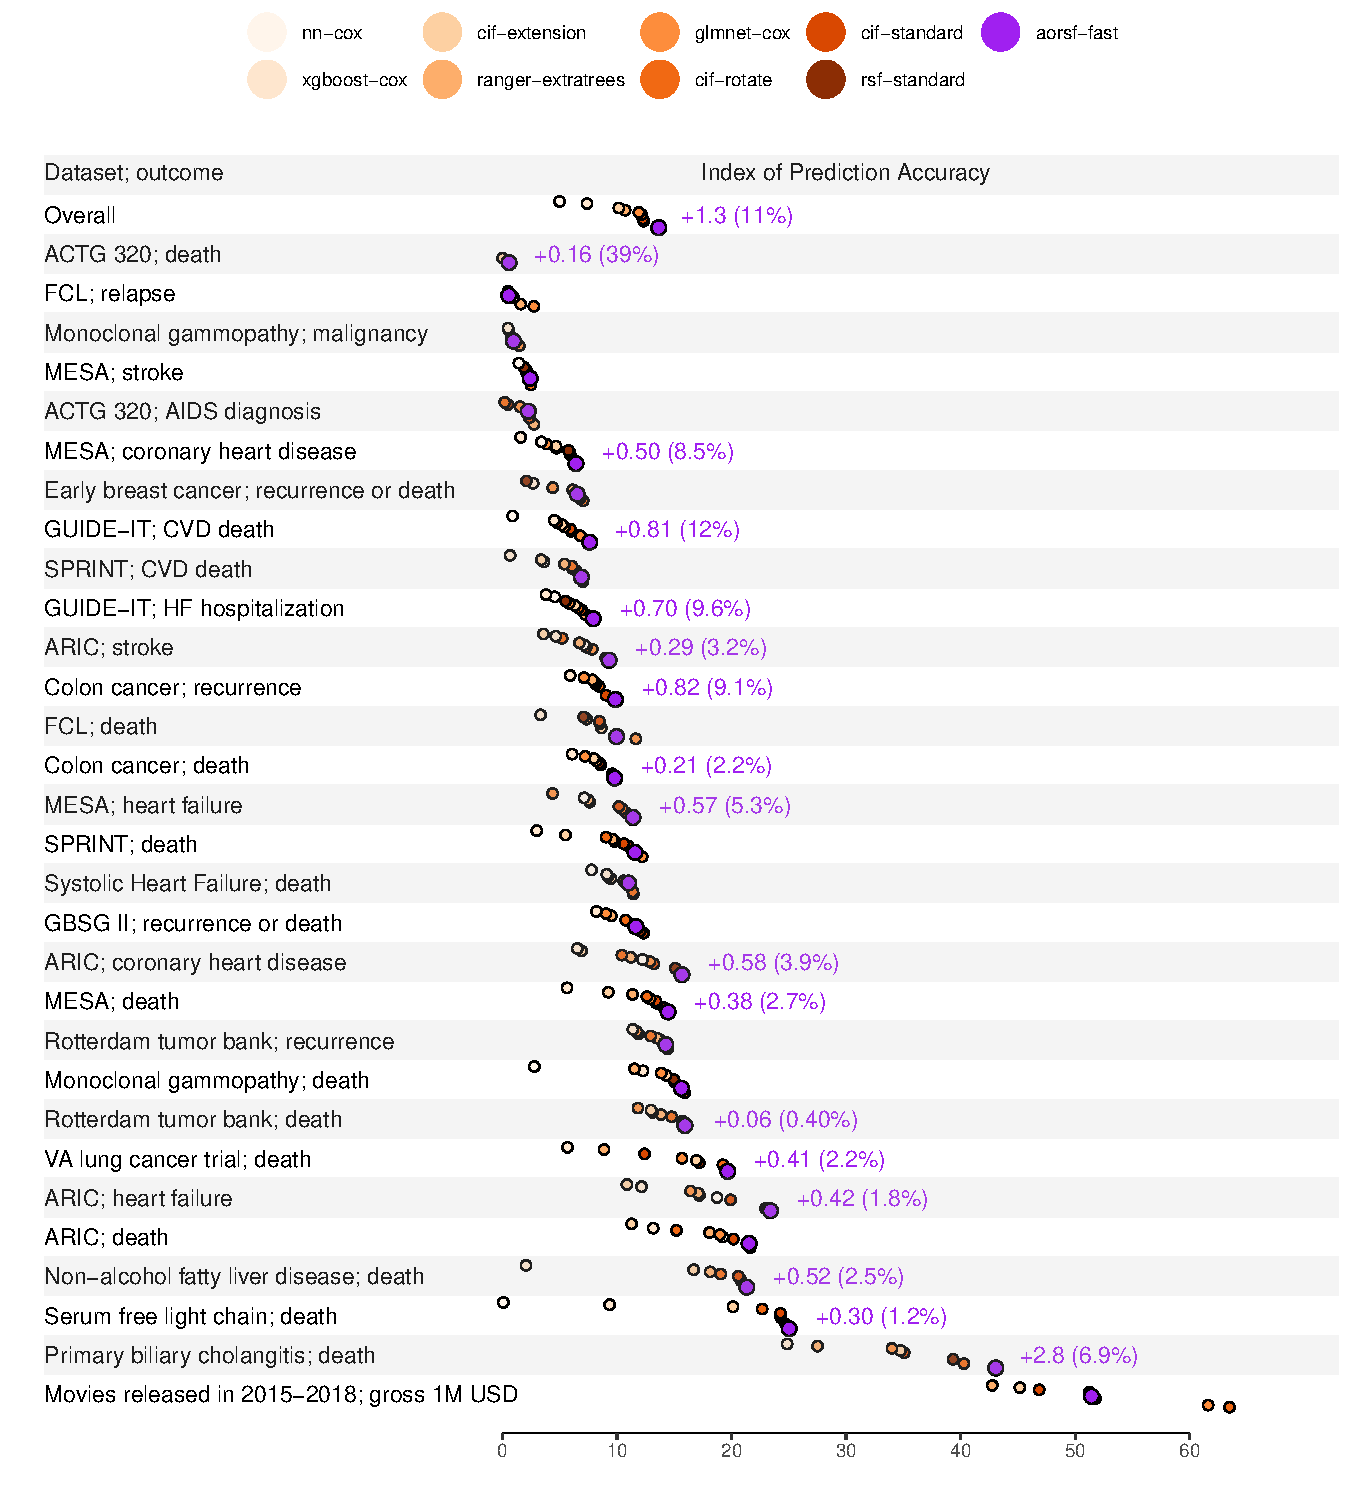
\includegraphics[width=\maxwidth]{figure/bm_pred_viz_ibs-1} \caption[Index of prediction accuracy for the accelerated oblique random survival forest and other learning algorithms across multiple risk prediction tasks]{Index of prediction accuracy for the accelerated oblique random survival forest and other learning algorithms across multiple risk prediction tasks. Text appears in tasks where the accelerated oblique random survival forest obtained the highest index of prediction accuracy, showing the absolute and percent improvement over the second best learner.}\label{fig:bm_pred_viz_ibs}
\end{figure}

\end{knitrout}


\begin{knitrout}
\definecolor{shadecolor}{rgb}{0.969, 0.969, 0.969}\color{fgcolor}\begin{figure}
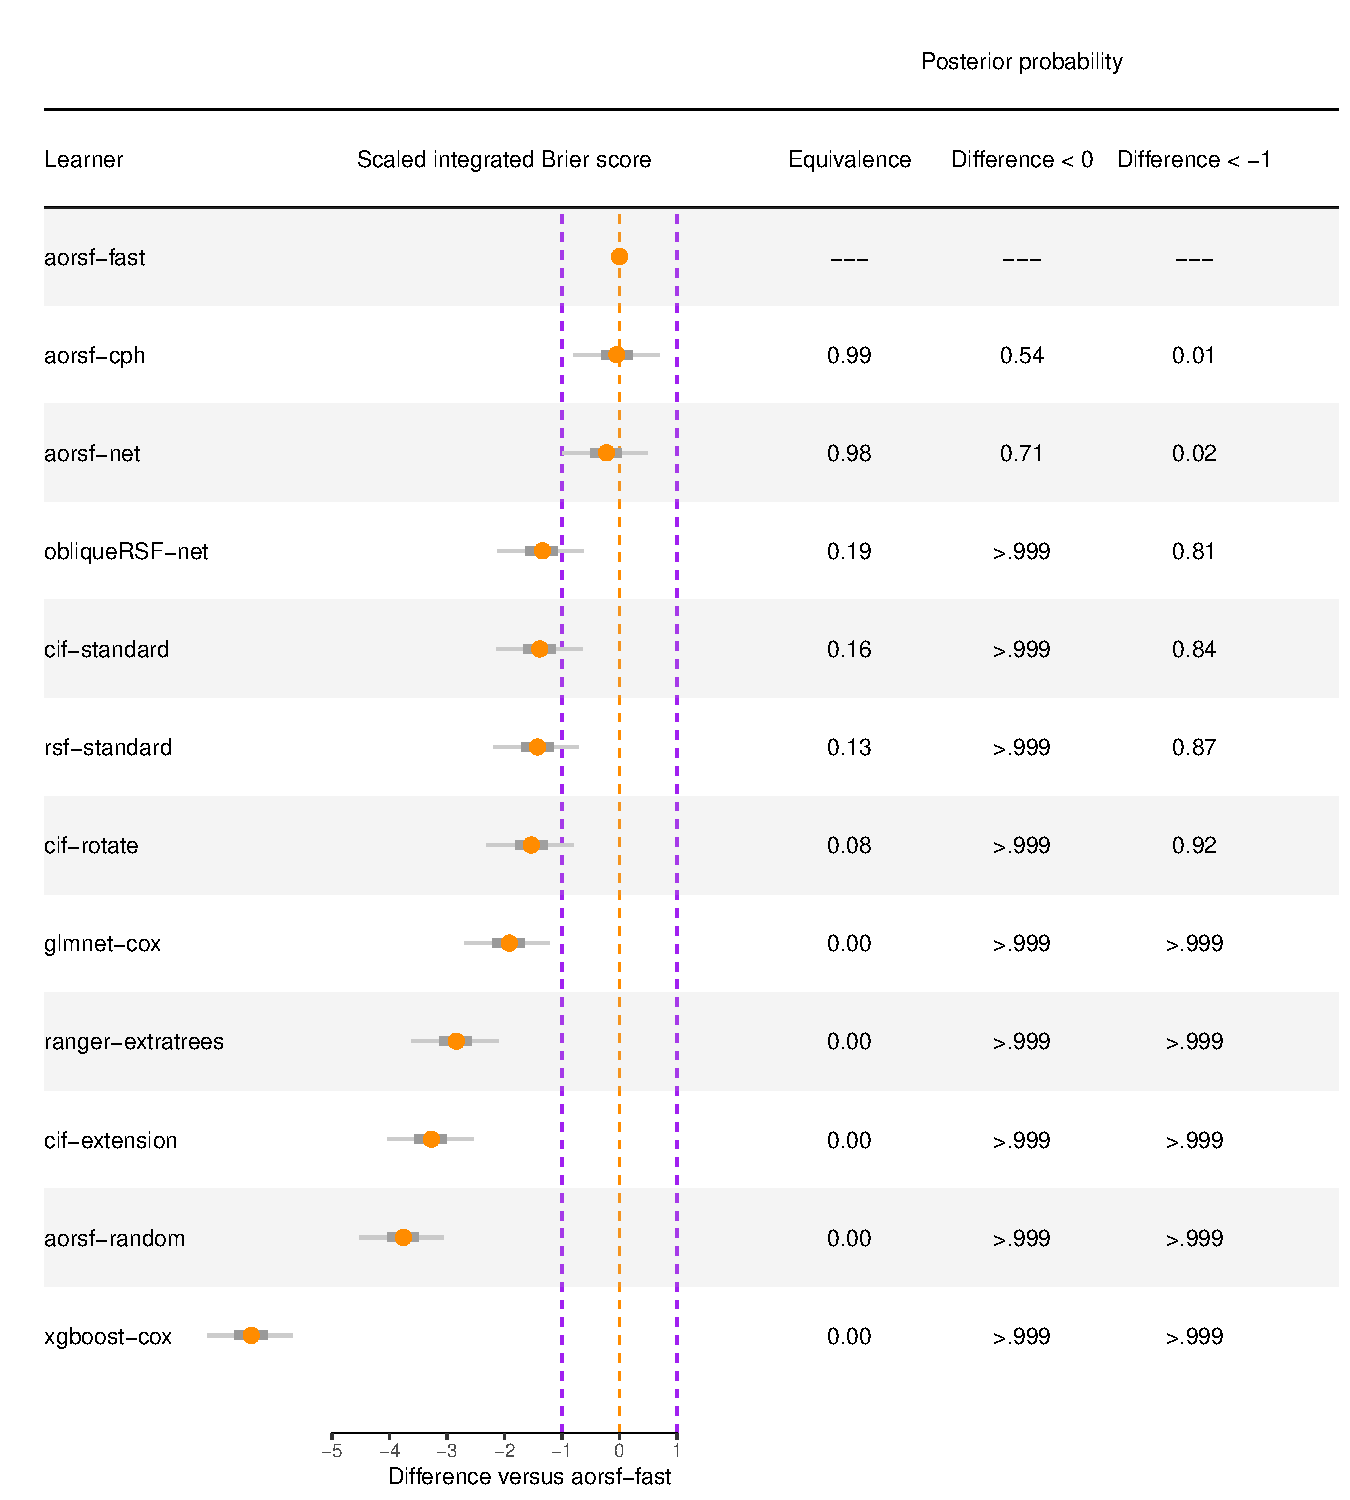
\includegraphics[width=\maxwidth]{figure/bm_pred_model_viz_ibs-1} \caption[Expected differences in index of prediction accuracy between the accelerated oblique random survival forest and other learning algorithms]{Expected differences in index of prediction accuracy between the accelerated oblique random survival forest and other learning algorithms. A region of practical equivalence is shown by purple dotted lines, and a boundary of non-zero difference is shown by an orange dotted line at the origin.}\label{fig:bm_pred_model_viz_ibs}
\end{figure}

\end{knitrout}

\paragraph{Time-dependent concordance statistic}




Compared to learners that were not oblique RSFs, \texttt{aorsf-fast} had the highest time-dependent C-statistic in  out of 31 risk prediction tasks, with an overall mean of  (Figure \ref{fig:bm_pred_viz_cstat}). Compared to the learner with the second highest mean C-statistic (\texttt{obliqueRSF-net}), \texttt{aorsf-fast}'s mean was 0.612 points higher, a relative increase of 0.797\%. The posterior probability of \texttt{aorsf-fast} and \texttt{aorsf-cph} having practically equivalent expected time-dependent C-statistics was 0.96, and the posterior probability of \texttt{aorsf-fast} having a superior time-dependent C-statistic versus other learners ranged from 0.02 (versus \texttt{obliqueRSF-net}) to $>$0.999 (versus several other learners; see Figure \ref{fig:bm_pred_model_viz_cstat})

\begin{knitrout}
\definecolor{shadecolor}{rgb}{0.969, 0.969, 0.969}\color{fgcolor}\begin{figure}
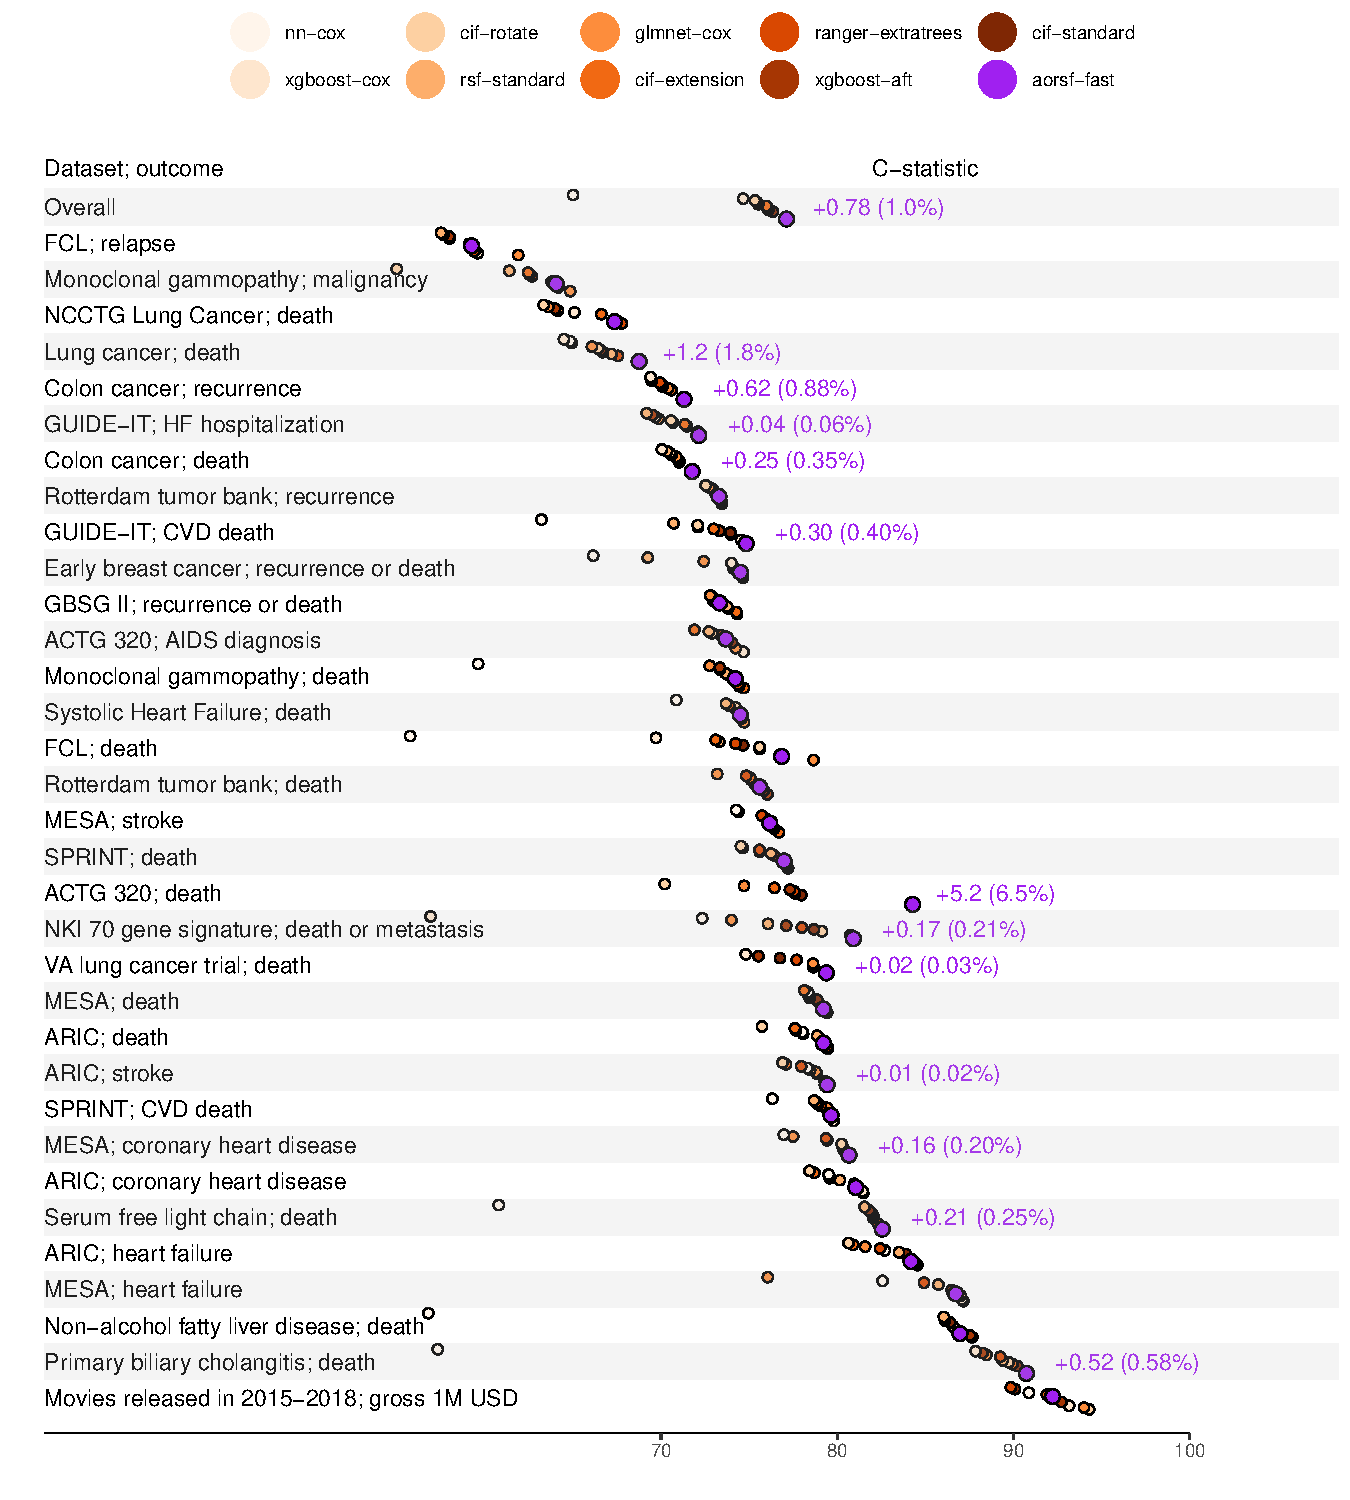
\includegraphics[width=\maxwidth]{figure/bm_pred_viz_cstat-1} \caption[Time-dependent concordance statistic for the accelerated oblique random survival forest and other learning algorithms across multiple risk prediction tasks]{Time-dependent concordance statistic for the accelerated oblique random survival forest and other learning algorithms across multiple risk prediction tasks. Text appears in tasks where the accelerated oblique random survival forest obtained the highest concordance, showing the absolute and percent improvement over the second best learner.}\label{fig:bm_pred_viz_cstat}
\end{figure}

\end{knitrout}


\begin{knitrout}
\definecolor{shadecolor}{rgb}{0.969, 0.969, 0.969}\color{fgcolor}\begin{figure}
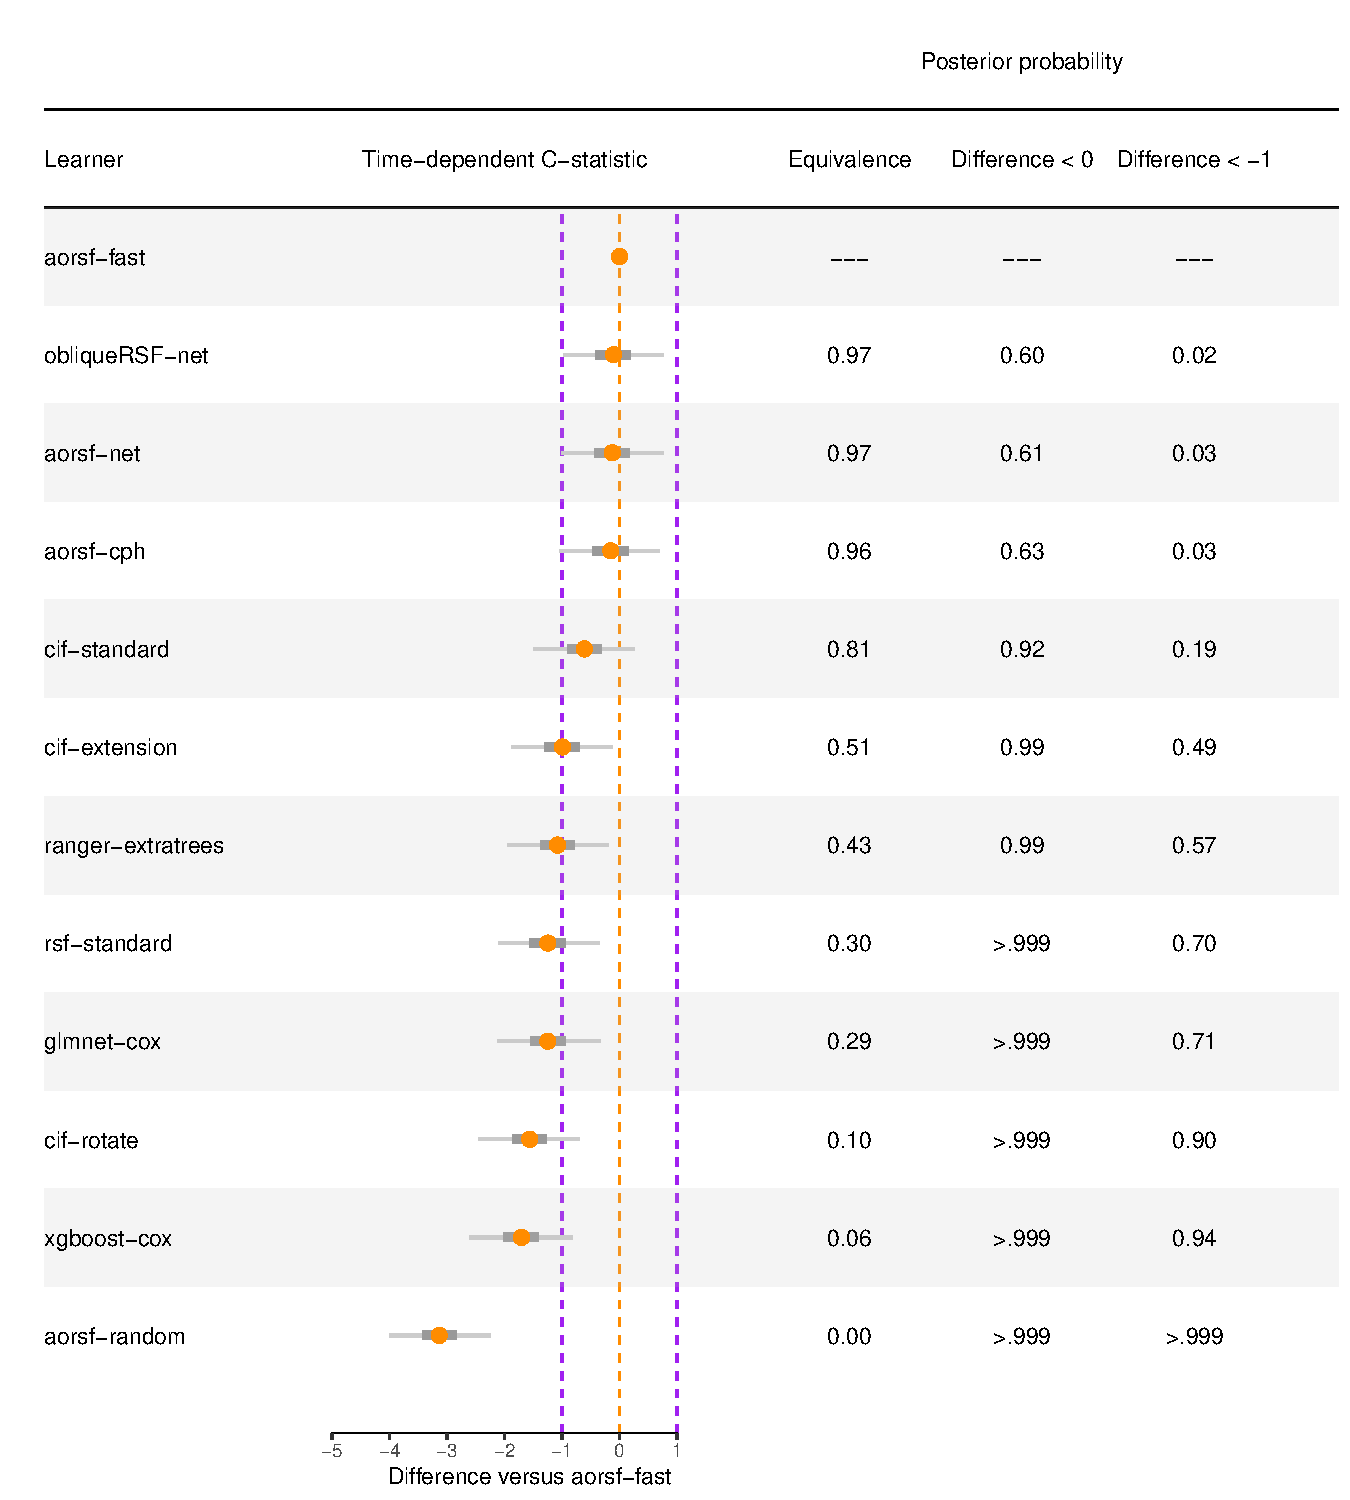
\includegraphics[width=\maxwidth]{figure/bm_pred_model_viz_cstat-1} \caption[Expected differences in time-dependent concordance statistic between the accelerated oblique random survival forest and other learning algorithms]{Expected differences in time-dependent concordance statistic between the accelerated oblique random survival forest and other learning algorithms. A region of practical equivalence is shown by purple dotted lines, and a boundary of non-zero difference is shown by an orange dotted line at the origin.}\label{fig:bm_pred_model_viz_cstat}
\end{figure}

\end{knitrout}

\paragraph{Computational efficiency}

Overall, \texttt{aorsf-fast} was the second fastest learner, with an expected model development and risk prediction time about 1/2 second longer than \texttt{glmnet-cox} (Figure \ref{fig:bm_pred_time}). Compared to its predecessor, \texttt{obliqueRSF-net}, \texttt{aorsf-fast} was XYZ times faster.



\begin{knitrout}
\definecolor{shadecolor}{rgb}{0.969, 0.969, 0.969}\color{fgcolor}\begin{figure}
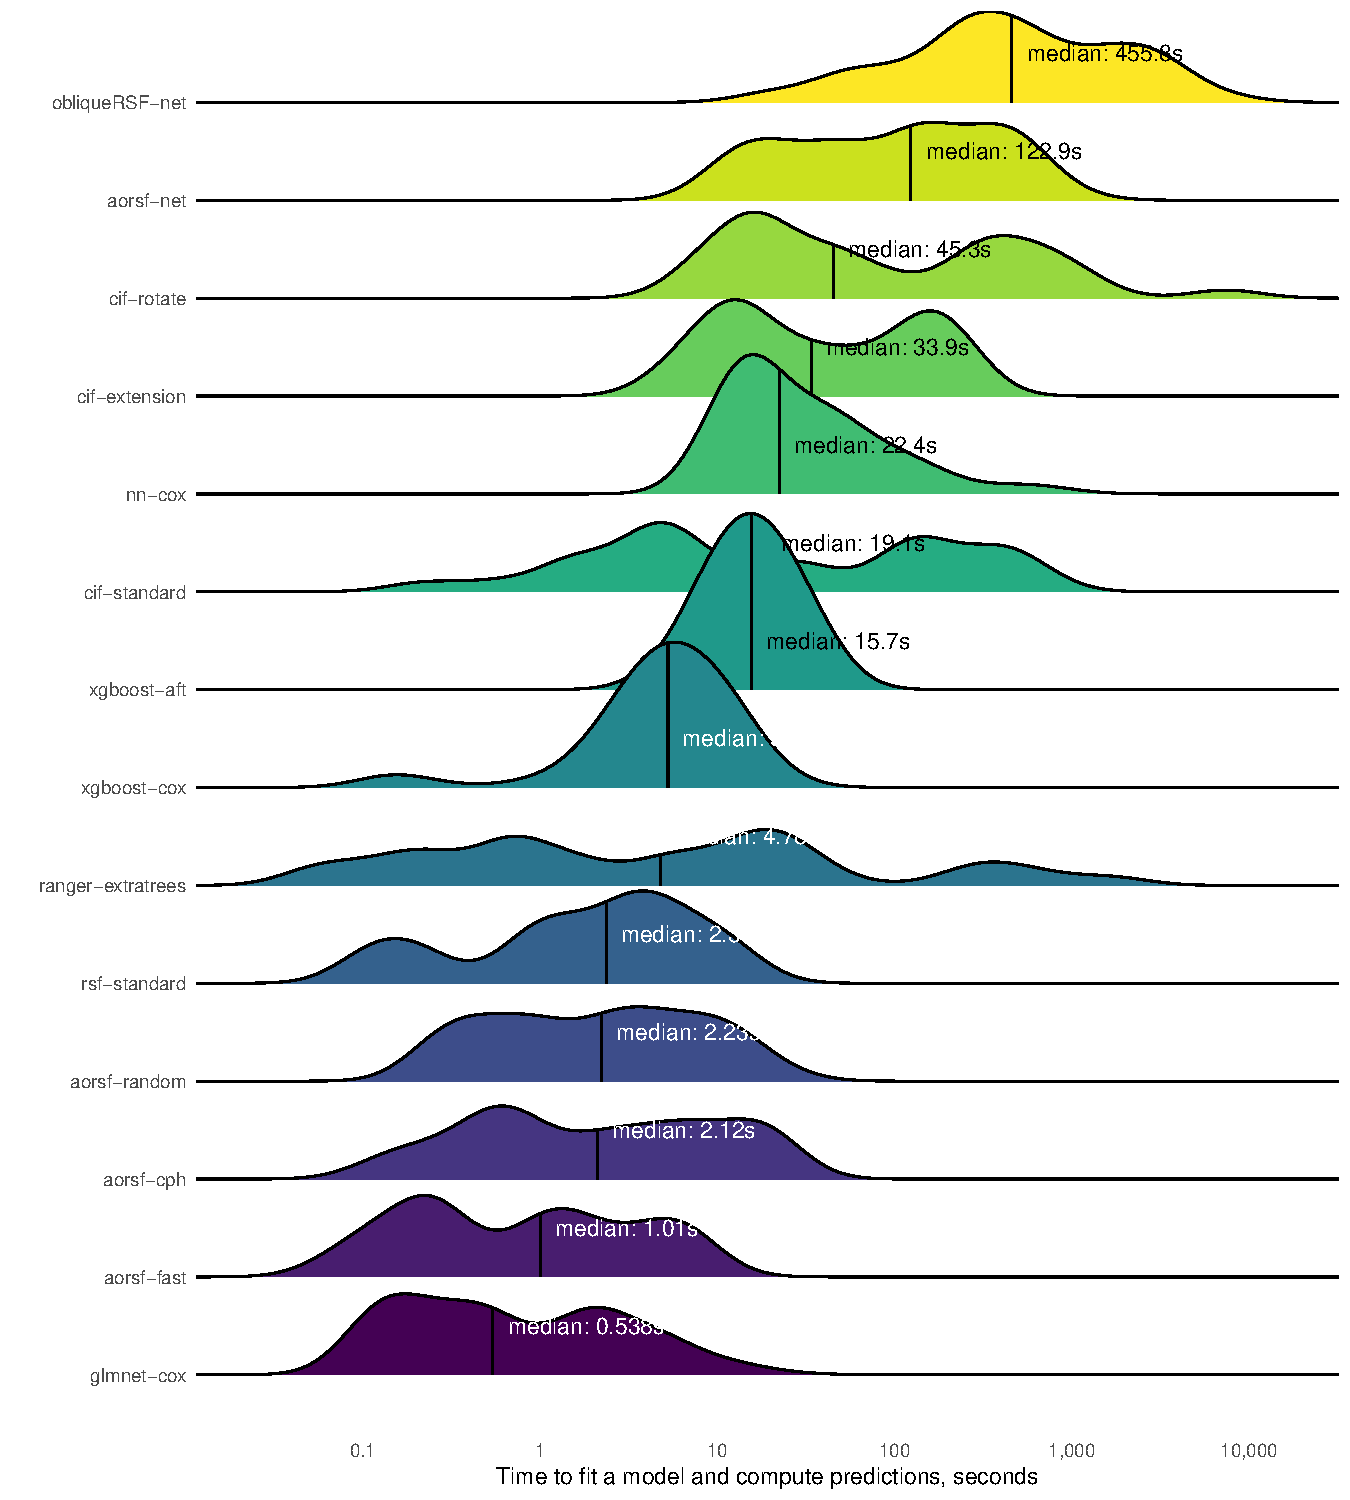
\includegraphics[width=\maxwidth]{figure/bm_pred_time-1} \caption[Distribution of time taken to fit a prediction model and compute predicted risk]{Distribution of time taken to fit a prediction model and compute predicted risk. The median time, in seconds, is printed and annotated for each learner by a vertical line.}\label{fig:bm_pred_time}
\end{figure}

\end{knitrout}


\subsection{Benchmark of variable importance}

The aim of this experiment is to evaluate negation VI and similar VI methods based on how well they can discriminate between variables that do or do not have a relationship with a simulated outcome. We consider methods that are intrinsic to the oblique RF (\eg ANOVA VI), those that are intrinsic to the RF (\eg permutation VI), and those that are model-agnostic (\eg SHAP VI).

\subsubsection{Variable importance techniques}

We compute permutation VI for axis based RSFs using the \texttt{randomForestSRC} package. Although the \texttt{party} package implements the approach to VI developed by \citet{strobl2007bias}, the developers of the \texttt{party} package note that the implementation of this approach for survival outcomes is ``extremely slow and experimental'' as of version 1.3.10. Therefore, it is not incorporated in the current simulation study. We compute ANOVA VI, negation VI, and permutation VI for oblique RSFs using the \texttt{aorsf} package. For ANOVA VI, we applied a p-value threshold of 0.01, following the threshold recommended by \citet{menze2011oblique}. We compute SHAP VI for boosted tree models using the \texttt{xgboost} package, which incorporates the tree SHAP approach proposed by \citet{lundberg2018consistent}. We also compute SHAP VI for accelerated oblique RSFs using the \texttt{fastshap} package.

\subsubsection{Variable types}

We considered five classes of predictor variables, with each class characterized by its variables' relationship to a right-censored outcome. Specifically, \begin{itemize}
\item \textit{irrelevant} variables had no relationship with the outcome.
\item \textit{main effect} variables had a linear relationship to the outcome.
\item \textit{non-linear effect} variables had a non-linear relationship to the outcome.
\item \textit{combination effect} variables were formed by linear combinations of three other variables. While their combination was linearly related to the outcome, each of the three variables contributing to the combination had no relation to the outcome.
\item \textit{interaction effect} variables were related to the outcome by multiplicative interaction with one other variable, which could have been a main effect, non-linear effect, or combination effect variable.
\end{itemize}


\subsubsection{Simulated data}

We initiated each set of simulated data with a random draw of size $n$ from a $p$-dimensional multivariate normal distribution, yielding $n$ observations of $p$ predictors. Each of $p$ predictor variables had a mean of zero, standard deviation of 1, and correlation with other predictor variables drawn at random between a lower and upper boundary. A time-to-event outcome with roughly 45\% of observations censored was generated using the \texttt{simsurv} package. The full predictor matrix (\ie, including interactions, non-linear mappings, and combinations) was used to generate the outcome. Interactions, non-linear mappings, and combinations were dropped from the predictor matrix after the outcome was generated so that VI techniques could be valuated based on their ability to detect these effects.

\subsubsection{Parameter specifications}

Parameters that varied in the current simulation study included the number of observations (1000, 3000, and 5000) and the minimum and maximum correlation between predictors (-0.1 to 0.1, -0.3 to 0.3, and -0.5 to 0.5). Parameters that remain fixed throughout the study included the number of predictors in each class (15) and the effect size of each predictor, with an increase of one standard deviation associated with a 64\% increase in relative risk.

\subsubsection{Evaluation of variable importance}

We compared VI techniques based on their discrimination (\ie C-statistic) between relevant and irrelevant variables. Specifically, we generated a binary outcome for each predictor variable based on its relevance (\ie, the binary outcome is 1 if the variable is relevant, 0 otherwise). Treating VI as if it were a ‘prediction’ for these binary outcomes yields a C-statistic is interpreted as the probability that the VI technique will rank a relevant variable higher than an irrelevant variable \citep{harrell1982evaluating}.

\subsubsection{Results} \label{sec:results_vi}



Overall, \texttt{aorsf-negate} had the highest C-statistic in 21 out of 36 VI tasks, with an overall mean of 75.3 (Figure \ref{fig:bm_vi_viz}). Compared to the VI technique with the second highest overall C-statistic (\texttt{aorsf-anova}), \texttt{aorsf-negate}'s mean was 2.34 points higher, a relative increase of 3.21\%. Among each of the four relevant variable classes, \texttt{aorsf-negate} had the highest mean C-statistic, with the greatest advantage of using \texttt{aorsf-negate} occurring among non-linear and combination variables and the smallest advantage for interaction variables.

\begin{knitrout}
\definecolor{shadecolor}{rgb}{0.969, 0.969, 0.969}\color{fgcolor}\begin{figure}
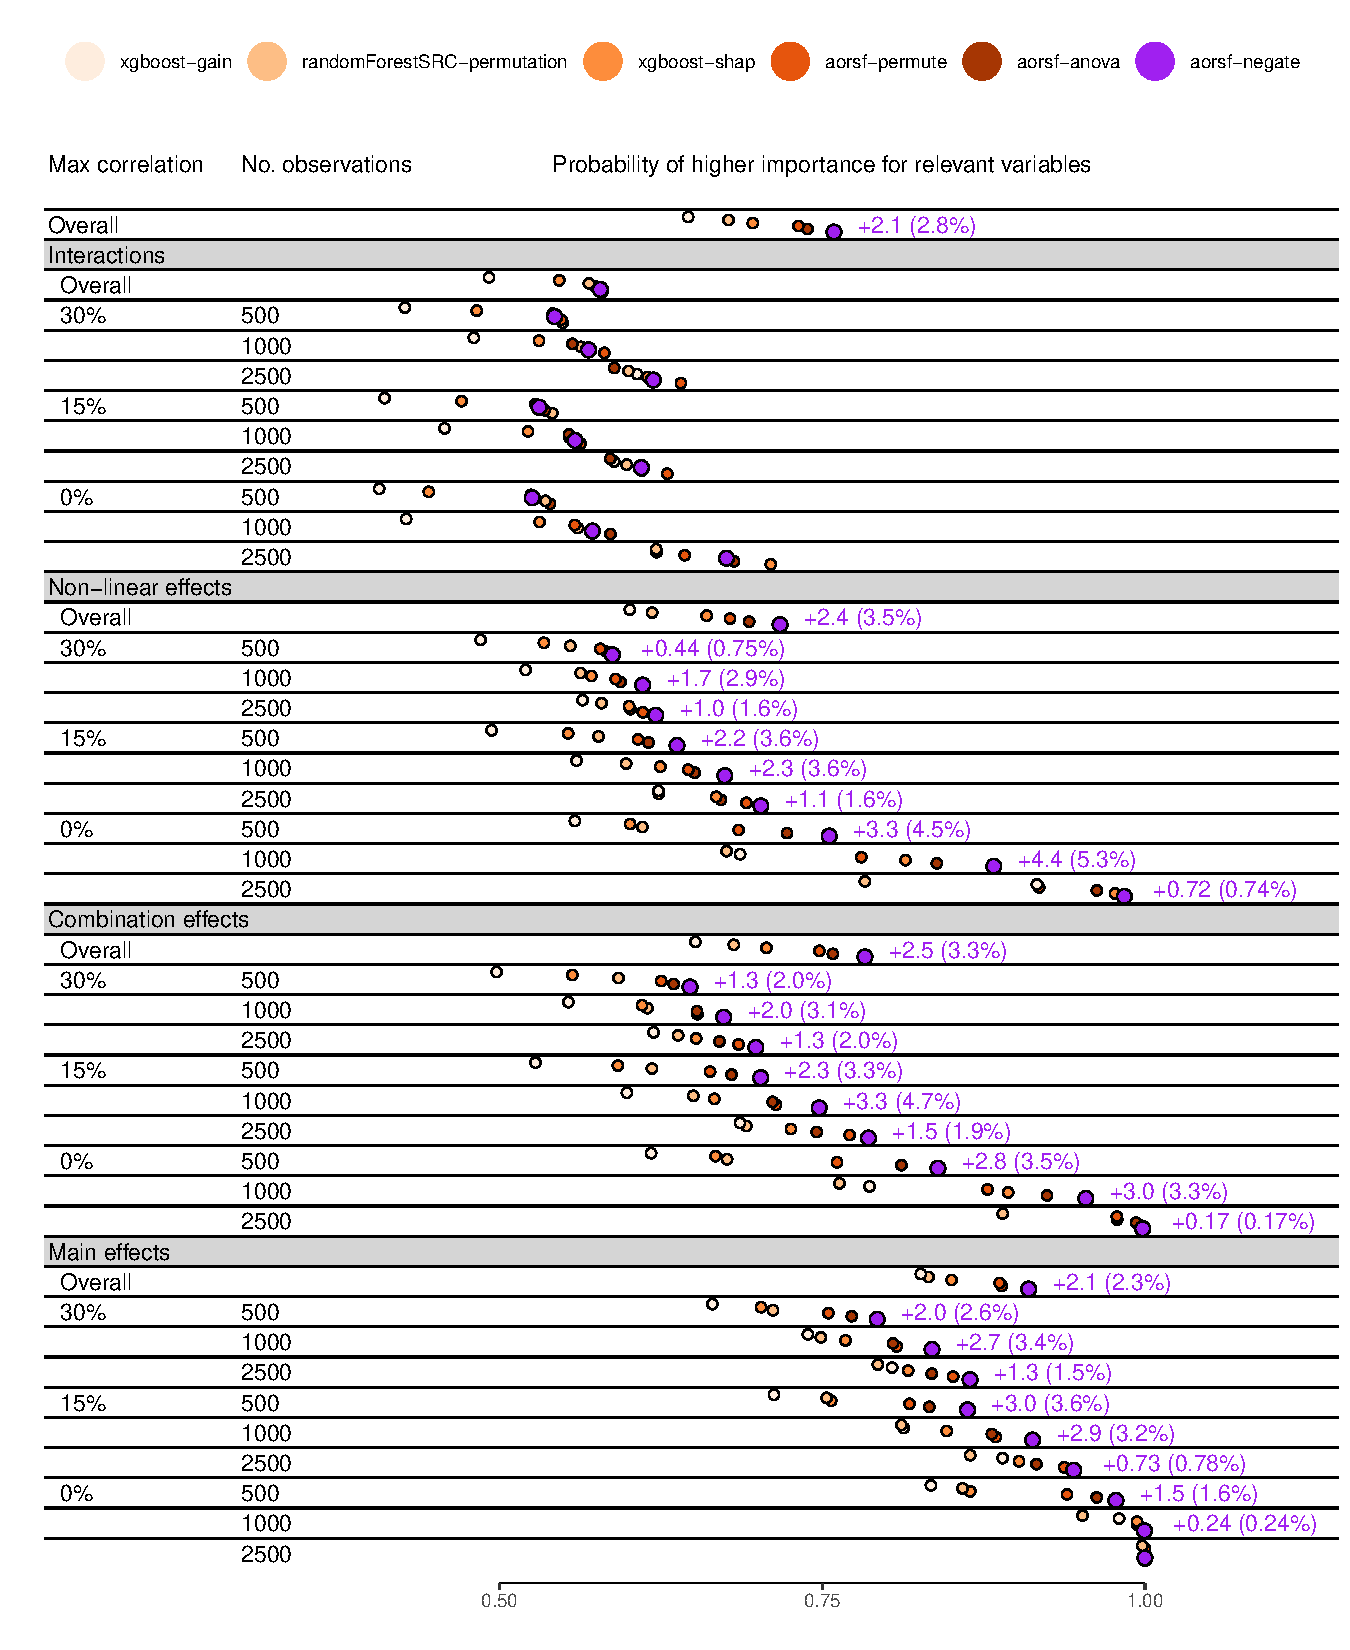
\includegraphics[width=\maxwidth]{figure/bm_vi_viz-1} \caption[Concordance statistic for assigning higher importance to relevant versus irrelevant variables]{Concordance statistic for assigning higher importance to relevant versus irrelevant variables. Text appears in rows where negation importance obtained the highest concordance, showing absolute and percent improvement over the second best technique.}\label{fig:bm_vi_viz}
\end{figure}

\end{knitrout}


\section{Discussion}

In this paper, we have developed two contributions to the oblique RSF: (1) the accelerated oblique RSF (\ie, \texttt{aorsf-fast}) and (2) negation VI. Our technique to accelerate the oblique RSF reduces the number of operations required to find linear combinations of inputs using a single iteration of Newton Raphson scoring, while our VI technique directly engages with coefficients in linear combinations of inputs to measure importance of individual variables. In numeric experiments, we found that that \texttt{aorsf-fast} is orders of magnitude more efficient and just as accurate in risk prediction tasks compared to its predecessor, \texttt{obliqueRSF-net}. We also found several cases where negation VI allows oblique RSF models to discriminate between relevant and irrelevant variables more effectively than three standard methods to estimate VI: permutation, ANOVA, and SHAP VI. Our results favored negation VI in scenarios where oblique RSFs were the underlying model used to compute VI and also in scenarios where other modeling techniques (\eg, boosted tree ensembles) were used.

\subsection{Implications of our results}

Accurate risk prediction models have the potential to improve healthcare by directing timely interventions to patients who are most likely to benefit. However, prediction models that cannot be interpreted and explained have no place in clinical practice. The current study advances the oblique RSF, an accurate risk prediction model, several steps towards being an accurate \textit{and} interpretable risk prediction model. The improved computational efficiency of the accelerated oblique RSF increases the feasibility of applying model-agnostic methods (\eg, SHAP values) for interpretation. Faster model evaluation and re-fitting also improve diagnosis and resolution of model-based issues (\eg, model calibration deteriorates over time). The introduction of negation VI also advances interpretability. VI is intrinsically linked to model fairness, as it can be used to identify when protected characteristics such as race, religion, and sexuality are inadvertently used (either directly or through correlates of these characteristics) by a prediction model. Since negation VI  engages with the coefficients used in linear combinations of variables, a major component of oblique RSFs, it may be more capable of diagnosing unfairness in oblique RSFs compared to permutation importance and model-agnostic VI techniques.

\subsection{Limitations and next steps}

The current study has several limitations. The accelerated oblique RSF does not account for competing risks, and so our benchmark of prediction accuracy divided tasks where competing risks were present into event-specific tasks. Biased estimation of incidence may occur when competing risks are ignored, and allowing the oblique RSF to account for competing risks is a high priority for future studies. In addition, missing data are not addressed in the accelerated oblique RSF, and users are expected to impute missing values before passing training or testing data into exported functions from the \texttt{aorsf} R package. However, missing data are common and it is standard for ensemble tree methods to handle missing data during the tree growing procedure. Thus, a second item of high priority for future studies is to develop and evaluate strategies to handle missing data while growing an oblique RSF.

% Acknowledgements should go at the end, before appendices and references

\acks{Research reported in this publication was supported by the Center for Biomedical Informatics, Wake Forest University School of Medicine. The project described was supported by the National Center for Advancing Translational Sciences (NCATS), National Institutes of Health, through Grant Award Number UL1TR001420. The content is solely the responsibility of the authors and does not necessarily represent the official views of the NIH.}

% Manual newpage inserted to improve layout of sample file - not
% needed in general before appendices/bibliography.

\newpage

\appendix

\section*{Appendix}
\captionsetup{labelformat=AppendixTables}
\setcounter{table}{0}

\begin{knitrout}
\definecolor{shadecolor}{rgb}{0.969, 0.969, 0.969}\color{fgcolor}
\begin{landscape}
\begin{longtable}[t]{lcclcc}
\caption{\label{tab:unnamed-chunk-5}Data sets used for numeric experiments \label{tab:datasets}}\\
\toprule
Label & N observations & N predictors & Outcome & N Events & \% Censored\\
\midrule
VA lung cancer trial & 137 & 8 & Death & 128 & 6.57\\
\cmidrule{1-6}\pagebreak[0]
 &  &  & Recurrence & 468 & 49.6\\
\cmidrule{4-6}\nopagebreak
\multirow{-2}{*}{\raggedright\arraybackslash Colon cancer} & \multirow{-2}{*}{\centering\arraybackslash 929} & \multirow{-2}{*}{\centering\arraybackslash 12} & Death & 452 & 51.3\\
\cmidrule{1-6}\pagebreak[0]
Primary biliary cholangitis & 276 & 19 & Death & 111 & 59.8\\
\cmidrule{1-6}\pagebreak[0]
Movies released in 2015-2018 & 551 & 46 & Gross 1M USD & 522 & 5.26\\
\cmidrule{1-6}\pagebreak[0]
GBSG II & 686 & 10 & Recurrence Or Death & 299 & 56.4\\
\cmidrule{1-6}\pagebreak[0]
Systolic Heart Failure & 2,231 & 41 & Death & 726 & 67.5\\
\cmidrule{1-6}\pagebreak[0]
Serum free light chain & 7,874 & 10 & Death & 2,169 & 72.5\\
\cmidrule{1-6}\pagebreak[0]
Non-alcohol fatty liver disease & 17,549 & 24 & Death & 1,364 & 92.2\\
\cmidrule{1-6}\pagebreak[0]
 &  &  & Recurrence & 1,518 & 49.1\\
\cmidrule{4-6}\nopagebreak
\multirow{-2}{*}{\raggedright\arraybackslash Rotterdam tumor bank} & \multirow{-2}{*}{\centering\arraybackslash 2,982} & \multirow{-2}{*}{\centering\arraybackslash 11} & Death & 1,272 & 57.3\\
\cmidrule{1-6}\pagebreak[0]
 &  &  & AIDS Diagnosis & 96 & 91.7\\
\cmidrule{4-6}\nopagebreak
\multirow{-2}{*}{\raggedright\arraybackslash ACTG 320} & \multirow{-2}{*}{\centering\arraybackslash 1,151} & \multirow{-2}{*}{\centering\arraybackslash 12} & Death & 26 & 97.7\\
\cmidrule{1-6}\pagebreak[0]
 &  &  & Cardiovascular Death & 110 & 87.7\\
\cmidrule{4-6}\nopagebreak
\multirow{-2}{*}{\raggedright\arraybackslash GUIDE-IT} & \multirow{-2}{*}{\centering\arraybackslash 894} & \multirow{-2}{*}{\centering\arraybackslash 59} & Hf Hospitalization & 288 & 67.8\\
\cmidrule{1-6}\pagebreak[0]
Early breast cancer & 614 & 1,692 & Recurrence Or Death & 134 & 78.2\\
\cmidrule{1-6}\pagebreak[0]
 &  &  & Cardiovascular Death & 521 & 94.4\\
\cmidrule{4-6}\nopagebreak
\multirow{-2}{*}{\raggedright\arraybackslash SPRINT} & \multirow{-2}{*}{\centering\arraybackslash 9,361} & \multirow{-2}{*}{\centering\arraybackslash 174} & Death & 1,644 & 82.4\\
\cmidrule{1-6}\pagebreak[0]
Heart Transplant & 3,787 & 52 & Graft-Loss Or Death & 500 & 86.8\\
\cmidrule{1-6}\pagebreak[0]
 &  &  & Death & 76 & 86.0\\
\cmidrule{4-6}\nopagebreak
\multirow{-2}{*}{\raggedright\arraybackslash FCL} & \multirow{-2}{*}{\centering\arraybackslash 541} & \multirow{-2}{*}{\centering\arraybackslash 7} & Relapse & 272 & 49.7\\
\cmidrule{1-6}\pagebreak[0]
 &  &  & Death & 963 & 30.4\\
\cmidrule{4-6}\nopagebreak
\multirow{-2}{*}{\raggedright\arraybackslash Monoclonal gammopathy} & \multirow{-2}{*}{\centering\arraybackslash 1,384} & \multirow{-2}{*}{\centering\arraybackslash 8} & Malignancy & 115 & 91.7\\
\cmidrule{1-6}\pagebreak[0]
 &  &  & Heart Failure & 339 & 95.0\\
\cmidrule{4-6}\nopagebreak
 &  &  & Coronary Heart Disease & 439 & 93.5\\
\cmidrule{4-6}\nopagebreak
 &  &  & Stroke & 292 & 95.7\\
\cmidrule{4-6}\nopagebreak
\multirow{-4}{*}{\raggedright\arraybackslash MESA} & \multirow{-4}{*}{\centering\arraybackslash 6,783} & \multirow{-4}{*}{\centering\arraybackslash 48} & Death & 1,297 & 80.9\\
\cmidrule{1-6}\pagebreak[0]
 &  &  & Heart Failure & 2,981 & 78.1\\
\cmidrule{4-6}\nopagebreak
 &  &  & Coronary Heart Disease & 2,282 & 83.2\\
\cmidrule{4-6}\nopagebreak
 &  &  & Stroke & 1,323 & 90.3\\
\cmidrule{4-6}\nopagebreak
\multirow{-4}{*}{\raggedright\arraybackslash ARIC} & \multirow{-4}{*}{\centering\arraybackslash 13,623} & \multirow{-4}{*}{\centering\arraybackslash 41} & Death & 6,662 & 51.1\\
\bottomrule
\end{longtable}
\end{landscape}

\end{knitrout}

\newpage

\begin{knitrout}
\definecolor{shadecolor}{rgb}{0.969, 0.969, 0.969}\color{fgcolor}
\begin{longtable}[t]{lcclc}
\caption{\label{tab:unnamed-chunk-6}Index of prediction accuracy, time-dependent concordance statistic, and computational time required to fit and compute predictions for several learning algorithms across 31 risk prediction tasks.}\\
\toprule
\multicolumn{1}{c}{ } & \multicolumn{2}{c}{Performance metric (SD)} & \multicolumn{2}{c}{Computation time, seconds} \\
\cmidrule(l{3pt}r{3pt}){2-3} \cmidrule(l{3pt}r{3pt}){4-5}
  & Scaled Brier & C-Statistic & Model fitting & Risk prediction\\
\midrule
\endfirsthead
\caption[]{Index of prediction accuracy, time-dependent concordance statistic, and computational time required to fit and compute predictions for several learning algorithms across 31 risk prediction tasks. \textit{(continued)}}\\
\toprule
  & Scaled Brier & C-Statistic & Model fitting & Risk prediction\\
\midrule
\endhead

\endfoot
\bottomrule
\endlastfoot
\addlinespace[0.3em]
\hline
\multicolumn{5}{l}{\textit{\textbf{Overall}}}\\
\hline
\hspace{1em}aorsf-fast & 0.132 (0.114) & 0.774 (0.072) & 0.833 & 0.173\\
\hspace{1em}aorsf-cph & 0.131 (0.115) & 0.772 (0.072) & 2.477 & 0.174\\
\hspace{1em}aorsf-net & 0.130 (0.118) & 0.772 (0.072) & 131.969 & 0.176\\
\hspace{1em}rsf-standard & 0.121 (0.118) & 0.761 (0.075) & 2.070 & 0.291\\
\hspace{1em}cif-standard & 0.120 (0.101) & 0.768 (0.071) & 4.499 & 15.774\\
\hspace{1em}cif-rotate & 0.119 (0.129) & 0.758 (0.080) & 43.469 & 9.418\\
\hspace{1em}obliqueRSF-net & 0.119 (0.088) & 0.773 (0.071) & 388.086 & 24.864\\
\hspace{1em}glmnet-cox & 0.115 (0.123) & 0.761 (0.074) & 0.693 & 0.004\\
\hspace{1em}ranger-extratrees & 0.104 (0.090) & 0.763 (0.068) & 2.147 & 1.592\\
\hspace{1em}cif-extension & 0.099 (0.095) & 0.764 (0.072) & 23.953 & 8.487\\
\hspace{1em}aorsf-random & 0.095 (0.085) & 0.742 (0.065) & 2.288 & 0.174\\
\hspace{1em}xgboost-cox & 0.076 (0.105) & 0.757 (0.088) & 4.399 & 0.005\\
\hspace{1em}nn-cox & 0.045 (0.101) & 0.648 (0.137) & 16.081 & 5.931\\
\hspace{1em}xgboost-aft & -4.80 (5.11) & 0.767 (0.077) & 14.692 & 0.007\\
\addlinespace[0.3em]
\hline
\multicolumn{5}{l}{\textit{\textbf{ACTG 320; AIDS diagnosis, n = 1151, p = 12}}}\\
\hline
\hspace{1em}ranger-extratrees & 0.028 (0.018) & 0.737 (0.042) & 0.053 & 0.155\\
\hspace{1em}aorsf-random & 0.024 (0.019) & 0.732 (0.042) & 0.452 & 0.036\\
\hspace{1em}cif-standard & 0.024 (0.039) & 0.741 (0.060) & 1.460 & 4.523\\
\hspace{1em}cif-extension & 0.022 (0.021) & 0.716 (0.055) & 9.093 & 4.176\\
\hspace{1em}obliqueRSF-net & 0.020 (0.030) & 0.733 (0.056) & 26.723 & 16.653\\
\hspace{1em}aorsf-cph & 0.017 (0.032) & 0.736 (0.056) & 0.452 & 0.037\\
\hspace{1em}aorsf-fast & 0.016 (0.027) & 0.733 (0.054) & 0.153 & 0.034\\
\hspace{1em}glmnet-cox & 0.011 (0.023) & 0.735 (0.034) & 0.180 & 0.002\\
\hspace{1em}aorsf-net & 0.010 (0.041) & 0.731 (0.055) & 19.025 & 0.036\\
\hspace{1em}xgboost-cox & 0.006 (0.046) & 0.747 (0.052) & 3.312 & 0.003\\
\hspace{1em}rsf-standard & 0.004 (0.042) & 0.721 (0.058) & 0.466 & 0.061\\
\hspace{1em}nn-cox & 0.001 (0.007) & 0.589 (0.138) & 10.976 & 0.666\\
\hspace{1em}cif-rotate & -0.002 (0.050) & 0.728 (0.051) & 14.852 & 4.031\\
\hspace{1em}xgboost-aft & -7.31 (0.690) & 0.739 (0.040) & 9.771 & 0.006\\
\addlinespace[0.3em]
\hline
\multicolumn{5}{l}{\textit{\textbf{ACTG 320; death, n = 1151, p = 12}}}\\
\hline
\hspace{1em}cif-extension & 0.004 (0.012) & 0.794 (0.066) & 12.087 & 5.085\\
\hspace{1em}obliqueRSF-net & 0.003 (0.012) & 0.822 (0.064) & 8.856 & 11.019\\
\hspace{1em}aorsf-fast & 0.001 (0.019) & 0.830 (0.062) & 0.094 & 0.020\\
\hspace{1em}cif-standard & 0.000 (0.022) & 0.797 (0.079) & 1.505 & 4.550\\
\hspace{1em}aorsf-random & 0.000 (0.016) & 0.793 (0.090) & 0.247 & 0.023\\
\hspace{1em}aorsf-cph & -0.001 (0.018) & 0.811 (0.073) & 0.361 & 0.022\\
\hspace{1em}xgboost-cox & -0.005 (0.003) & 0.500 (0.000) & 0.116 & 0.002\\
\hspace{1em}nn-cox & -0.006 (0.003) & 0.514 (0.102) & 10.371 & 0.517\\
\hspace{1em}aorsf-net & -0.006 (0.034) & 0.813 (0.070) & 13.008 & 0.023\\
\hspace{1em}ranger-extratrees & -0.006 (0.022) & 0.768 (0.078) & 0.041 & 0.127\\
\hspace{1em}rsf-standard & -0.027 (0.060) & 0.796 (0.074) & 0.097 & 0.037\\
\hspace{1em}cif-rotate & -0.030 (0.037) & 0.727 (0.092) & 12.924 & 3.575\\
\hspace{1em}glmnet-cox & -0.057 (0.096) & 0.777 (0.062) & 0.282 & 0.003\\
\hspace{1em}xgboost-aft & -23.5 (7.27) & 0.772 (0.100) & 8.740 & 0.006\\
\addlinespace[0.3em]
\hline
\multicolumn{5}{l}{\textit{\textbf{ARIC; coronary heart disease, n = 13623, p = 41}}}\\
\hline
\hspace{1em}aorsf-fast & 0.156 (0.005) & 0.806 (0.004) & 4.321 & 1.354\\
\hspace{1em}aorsf-net & 0.153 (0.004) & 0.806 (0.003) & 515.337 & 1.480\\
\hspace{1em}aorsf-cph & 0.152 (0.005) & 0.806 (0.004) & 14.632 & 1.349\\
\hspace{1em}rsf-standard & 0.149 (0.006) & 0.797 (0.003) & 7.394 & 1.041\\
\hspace{1em}obliqueRSF-net & 0.145 (0.002) & 0.808 (0.002) & 3100.286 & 413.186\\
\hspace{1em}cif-standard & 0.133 (0.002) & 0.806 (0.002) & 69.980 & 358.577\\
\hspace{1em}glmnet-cox & 0.132 (0.008) & 0.795 (0.003) & 1.467 & 0.025\\
\hspace{1em}nn-cox & 0.123 (0.008) & 0.793 (0.004) & 82.973 & 106.367\\
\hspace{1em}ranger-extratrees & 0.112 (0.001) & 0.792 (0.003) & 271.533 & 63.785\\
\hspace{1em}cif-rotate & 0.106 (0.001) & 0.782 (0.006) & 578.571 & 68.467\\
\hspace{1em}aorsf-random & 0.098 (0.004) & 0.771 (0.004) & 11.278 & 1.387\\
\hspace{1em}cif-extension & 0.070 (0.001) & 0.784 (0.004) & 163.371 & 49.091\\
\hspace{1em}xgboost-cox & 0.062 (0.016) & 0.811 (0.004) & 8.980 & 0.014\\
\hspace{1em}xgboost-aft & -4.81 (0.208) & 0.812 (0.004) & 21.435 & 0.021\\
\addlinespace[0.3em]
\hline
\multicolumn{5}{l}{\textit{\textbf{ARIC; death, n = 13623, p = 41}}}\\
\hline
\hspace{1em}rsf-standard & 0.218 (0.004) & 0.790 (0.001) & 11.948 & 1.186\\
\hspace{1em}aorsf-net & 0.218 (0.006) & 0.792 (0.003) & 958.228 & 2.380\\
\hspace{1em}aorsf-cph & 0.215 (0.007) & 0.791 (0.003) & 22.614 & 2.249\\
\hspace{1em}aorsf-fast & 0.215 (0.007) & 0.792 (0.003) & 7.190 & 2.258\\
\hspace{1em}obliqueRSF-net & 0.208 (0.004) & 0.792 (0.003) & 7161.062 & 322.057\\
\hspace{1em}cif-standard & 0.202 (0.004) & 0.789 (0.004) & 64.173 & 379.745\\
\hspace{1em}glmnet-cox & 0.191 (0.017) & 0.777 (0.006) & 1.852 & 0.018\\
\hspace{1em}nn-cox & 0.183 (0.016) & 0.781 (0.003) & 95.577 & 77.835\\
\hspace{1em}ranger-extratrees & 0.181 (0.006) & 0.779 (0.005) & 350.659 & 58.944\\
\hspace{1em}cif-rotate & 0.152 (0.005) & 0.755 (0.006) & 577.948 & 65.954\\
\hspace{1em}xgboost-cox & 0.134 (0.015) & 0.795 (0.001) & 11.789 & 0.015\\
\hspace{1em}aorsf-random & 0.130 (0.004) & 0.733 (0.003) & 18.944 & 1.995\\
\hspace{1em}cif-extension & 0.114 (0.001) & 0.775 (0.005) & 180.959 & 50.040\\
\hspace{1em}xgboost-aft & -1.63 (0.238) & 0.795 (0.002) & 25.690 & 0.014\\
\addlinespace[0.3em]
\hline
\multicolumn{5}{l}{\textit{\textbf{ARIC; heart failure, n = 13623, p = 41}}}\\
\hline
\hspace{1em}aorsf-fast & 0.236 (0.005) & 0.842 (0.006) & 5.253 & 1.671\\
\hspace{1em}rsf-standard & 0.231 (0.005) & 0.835 (0.004) & 10.275 & 1.254\\
\hspace{1em}aorsf-net & 0.231 (0.004) & 0.842 (0.005) & 628.786 & 1.736\\
\hspace{1em}aorsf-cph & 0.231 (0.006) & 0.842 (0.006) & 16.545 & 1.568\\
\hspace{1em}obliqueRSF-net & 0.215 (0.003) & 0.841 (0.005) & 3701.023 & 306.739\\
\hspace{1em}cif-standard & 0.200 (0.002) & 0.839 (0.005) & 67.705 & 364.696\\
\hspace{1em}nn-cox & 0.181 (0.029) & 0.823 (0.008) & 79.949 & 112.151\\
\hspace{1em}glmnet-cox & 0.179 (0.036) & 0.821 (0.010) & 1.899 & 0.012\\
\hspace{1em}ranger-extratrees & 0.173 (0.003) & 0.825 (0.006) & 260.123 & 63.679\\
\hspace{1em}cif-rotate & 0.171 (0.003) & 0.806 (0.005) & 581.803 & 66.846\\
\hspace{1em}aorsf-random & 0.141 (0.004) & 0.792 (0.004) & 13.281 & 1.509\\
\hspace{1em}xgboost-cox & 0.119 (0.009) & 0.844 (0.005) & 13.603 & 0.015\\
\hspace{1em}cif-extension & 0.110 (0.003) & 0.809 (0.006) & 167.897 & 48.511\\
\hspace{1em}xgboost-aft & -3.93 (0.269) & 0.843 (0.005) & 22.308 & 0.022\\
\addlinespace[0.3em]
\hline
\multicolumn{5}{l}{\textit{\textbf{ARIC; stroke, n = 13623, p = 41}}}\\
\hline
\hspace{1em}aorsf-fast & 0.094 (0.003) & 0.794 (0.003) & 3.786 & 1.160\\
\hspace{1em}rsf-standard & 0.092 (0.003) & 0.786 (0.005) & 5.225 & 0.875\\
\hspace{1em}aorsf-net & 0.091 (0.003) & 0.793 (0.004) & 411.476 & 1.233\\
\hspace{1em}aorsf-cph & 0.090 (0.003) & 0.792 (0.004) & 13.452 & 1.127\\
\hspace{1em}obliqueRSF-net & 0.082 (0.002) & 0.791 (0.004) & 1751.465 & 410.345\\
\hspace{1em}glmnet-cox & 0.079 (0.005) & 0.785 (0.004) & 1.493 & 0.011\\
\hspace{1em}cif-standard & 0.074 (0.002) & 0.788 (0.004) & 78.679 & 394.309\\
\hspace{1em}nn-cox & 0.072 (0.016) & 0.782 (0.008) & 28.811 & 84.991\\
\hspace{1em}ranger-extratrees & 0.068 (0.003) & 0.780 (0.006) & 310.500 & 70.135\\
\hspace{1em}aorsf-random & 0.059 (0.004) & 0.752 (0.007) & 9.207 & 1.136\\
\hspace{1em}cif-rotate & 0.052 (0.002) & 0.768 (0.009) & 614.088 & 69.548\\
\hspace{1em}xgboost-cox & 0.047 (0.012) & 0.792 (0.001) & 6.854 & 0.014\\
\hspace{1em}cif-extension & 0.036 (0.001) & 0.772 (0.007) & 163.803 & 49.613\\
\hspace{1em}xgboost-aft & -6.78 (0.231) & 0.791 (0.002) & 21.692 & 0.023\\
\addlinespace[0.3em]
\hline
\multicolumn{5}{l}{\textit{\textbf{Colon cancer; death, n = 929, p = 12}}}\\
\hline
\hspace{1em}aorsf-fast & 0.099 (0.018) & 0.718 (0.013) & 0.228 & 0.047\\
\hspace{1em}cif-standard & 0.099 (0.016) & 0.712 (0.013) & 1.158 & 3.454\\
\hspace{1em}aorsf-cph & 0.097 (0.018) & 0.716 (0.012) & 0.646 & 0.051\\
\hspace{1em}aorsf-net & 0.095 (0.014) & 0.716 (0.010) & 48.543 & 0.049\\
\hspace{1em}aorsf-random & 0.095 (0.009) & 0.717 (0.012) & 1.361 & 0.045\\
\hspace{1em}cif-rotate & 0.095 (0.020) & 0.712 (0.011) & 12.821 & 3.474\\
\hspace{1em}obliqueRSF-net & 0.089 (0.005) & 0.716 (0.010) & 250.693 & 16.565\\
\hspace{1em}rsf-standard & 0.084 (0.026) & 0.705 (0.008) & 1.193 & 0.135\\
\hspace{1em}cif-extension & 0.080 (0.007) & 0.708 (0.013) & 10.097 & 4.783\\
\hspace{1em}ranger-extratrees & 0.078 (0.010) & 0.709 (0.017) & 0.494 & 0.239\\
\hspace{1em}glmnet-cox & 0.076 (0.018) & 0.703 (0.024) & 0.112 & 0.002\\
\hspace{1em}xgboost-cox & 0.060 (0.006) & 0.699 (0.010) & 2.915 & 0.003\\
\hspace{1em}nn-cox & -0.005 (0.003) & 0.521 (0.030) & 12.067 & 1.890\\
\hspace{1em}xgboost-aft & -1.06 (0.351) & 0.707 (0.013) & 13.225 & 0.006\\
\addlinespace[0.3em]
\hline
\multicolumn{5}{l}{\textit{\textbf{Colon cancer; recurrence, n = 929, p = 12}}}\\
\hline
\hspace{1em}aorsf-fast & 0.097 (0.012) & 0.710 (0.009) & 0.227 & 0.055\\
\hspace{1em}aorsf-cph & 0.096 (0.011) & 0.709 (0.008) & 0.639 & 0.052\\
\hspace{1em}aorsf-net & 0.096 (0.016) & 0.710 (0.012) & 51.707 & 0.045\\
\hspace{1em}cif-standard & 0.093 (0.016) & 0.700 (0.016) & 1.060 & 3.235\\
\hspace{1em}cif-rotate & 0.092 (0.017) & 0.698 (0.016) & 12.951 & 3.530\\
\hspace{1em}obliqueRSF-net & 0.089 (0.007) & 0.708 (0.011) & 263.760 & 15.788\\
\hspace{1em}aorsf-random & 0.086 (0.005) & 0.702 (0.004) & 1.285 & 0.051\\
\hspace{1em}cif-extension & 0.082 (0.005) & 0.703 (0.010) & 8.427 & 3.628\\
\hspace{1em}rsf-standard & 0.081 (0.019) & 0.695 (0.012) & 1.290 & 0.145\\
\hspace{1em}ranger-extratrees & 0.075 (0.008) & 0.694 (0.010) & 0.562 & 0.225\\
\hspace{1em}glmnet-cox & 0.069 (0.012) & 0.692 (0.018) & 0.117 & 0.003\\
\hspace{1em}xgboost-cox & 0.056 (0.011) & 0.691 (0.012) & 3.446 & 0.003\\
\hspace{1em}nn-cox & -0.037 (0.064) & 0.519 (0.030) & 22.950 & 1.477\\
\hspace{1em}xgboost-aft & -1.20 (0.298) & 0.698 (0.015) & 11.457 & 0.006\\
\addlinespace[0.3em]
\hline
\multicolumn{5}{l}{\textit{\textbf{Early breast cancer; recurrence or death, n = 614, p = 1692}}}\\
\hline
\hspace{1em}obliqueRSF-net & 0.069 (0.036) & 0.755 (0.030) & 1875.318 & 12.911\\
\hspace{1em}cif-standard & 0.064 (0.027) & 0.752 (0.026) & 7.791 & 3.966\\
\hspace{1em}cif-rotate & 0.062 (0.021) & 0.741 (0.017) & 6623.673 & 366.471\\
\hspace{1em}cif-extension & 0.060 (0.021) & 0.748 (0.024) & 42.790 & 6.410\\
\hspace{1em}aorsf-cph & 0.057 (0.054) & 0.747 (0.019) & 1.313 & 0.169\\
\hspace{1em}aorsf-fast & 0.056 (0.054) & 0.749 (0.023) & 0.735 & 0.170\\
\hspace{1em}ranger-extratrees & 0.054 (0.043) & 0.746 (0.022) & 0.221 & 0.165\\
\hspace{1em}glmnet-cox & 0.026 (0.023) & 0.722 (0.019) & 5.768 & 0.007\\
\hspace{1em}xgboost-cox & 0.025 (0.027) & 0.741 (0.017) & 2.311 & 0.007\\
\hspace{1em}aorsf-random & 0.023 (0.023) & 0.706 (0.035) & 1.402 & 0.174\\
\hspace{1em}aorsf-net & 0.014 (0.110) & 0.754 (0.014) & 461.060 & 0.176\\
\hspace{1em}rsf-standard & 0.013 (0.073) & 0.698 (0.053) & 0.327 & 0.451\\
\hspace{1em}nn-cox & -0.039 (0.088) & 0.650 (0.075) & 16.127 & 1.654\\
\hspace{1em}xgboost-aft & -3.09 (1.10) & 0.749 (0.020) & 9.377 & 0.010\\
\addlinespace[0.3em]
\hline
\multicolumn{5}{l}{\textit{\textbf{FCL; death, n = 541, p = 7}}}\\
\hline
\hspace{1em}glmnet-cox & 0.117 (0.032) & 0.784 (0.045) & 0.096 & 0.002\\
\hspace{1em}aorsf-cph & 0.097 (0.055) & 0.774 (0.044) & 0.164 & 0.019\\
\hspace{1em}cif-extension & 0.097 (0.042) & 0.749 (0.045) & 5.240 & 2.305\\
\hspace{1em}aorsf-net & 0.095 (0.052) & 0.770 (0.040) & 12.784 & 0.018\\
\hspace{1em}aorsf-fast & 0.094 (0.053) & 0.774 (0.044) & 0.086 & 0.021\\
\hspace{1em}obliqueRSF-net & 0.090 (0.035) & 0.771 (0.047) & 101.477 & 5.378\\
\hspace{1em}rsf-standard & 0.090 (0.062) & 0.758 (0.042) & 0.562 & 0.038\\
\hspace{1em}aorsf-random & 0.086 (0.036) & 0.763 (0.049) & 0.296 & 0.019\\
\hspace{1em}cif-rotate & 0.085 (0.067) & 0.763 (0.036) & 6.328 & 2.376\\
\hspace{1em}cif-standard & 0.085 (0.049) & 0.755 (0.049) & 0.730 & 1.121\\
\hspace{1em}ranger-extratrees & 0.078 (0.017) & 0.752 (0.052) & 0.046 & 0.080\\
\hspace{1em}xgboost-cox & 0.047 (0.074) & 0.717 (0.119) & 2.504 & 0.002\\
\hspace{1em}nn-cox & 0.013 (0.041) & 0.493 (0.145) & 11.346 & 0.563\\
\hspace{1em}xgboost-aft & -2.48 (0.436) & 0.754 (0.057) & 6.730 & 0.005\\
\addlinespace[0.3em]
\hline
\multicolumn{5}{l}{\textit{\textbf{FCL; relapse, n = 541, p = 7}}}\\
\hline
\hspace{1em}glmnet-cox & 0.036 (0.023) & 0.625 (0.028) & 0.109 & 0.002\\
\hspace{1em}xgboost-cox & 0.023 (0.012) & 0.608 (0.029) & 1.694 & 0.002\\
\hspace{1em}obliqueRSF-net & 0.019 (0.018) & 0.593 (0.036) & 225.137 & 6.199\\
\hspace{1em}ranger-extratrees & 0.018 (0.023) & 0.586 (0.042) & 0.045 & 0.078\\
\hspace{1em}aorsf-random & 0.017 (0.027) & 0.594 (0.038) & 0.427 & 0.021\\
\hspace{1em}aorsf-cph & 0.011 (0.034) & 0.591 (0.040) & 0.318 & 0.026\\
\hspace{1em}aorsf-fast & 0.011 (0.033) & 0.589 (0.039) & 0.128 & 0.023\\
\hspace{1em}aorsf-net & 0.008 (0.036) & 0.587 (0.043) & 20.070 & 0.022\\
\hspace{1em}cif-standard & 0.006 (0.028) & 0.591 (0.034) & 0.721 & 1.132\\
\hspace{1em}nn-cox & -0.003 (0.030) & 0.534 (0.074) & 11.088 & 0.436\\
\hspace{1em}cif-extension & -0.004 (0.037) & 0.578 (0.045) & 6.192 & 2.357\\
\hspace{1em}cif-rotate & -0.008 (0.034) & 0.581 (0.036) & 7.111 & 2.207\\
\hspace{1em}rsf-standard & -0.025 (0.041) & 0.578 (0.038) & 1.326 & 0.086\\
\hspace{1em}xgboost-aft & -0.974 (0.221) & 0.574 (0.060) & 6.179 & 0.006\\
\addlinespace[0.3em]
\hline
\multicolumn{5}{l}{\textit{\textbf{GBSG II; recurrence or death, n = 686, p = 10}}}\\
\hline
\hspace{1em}cif-standard & 0.127 (0.013) & 0.748 (0.013) & 0.874 & 2.321\\
\hspace{1em}aorsf-net & 0.127 (0.018) & 0.745 (0.013) & 40.051 & 0.039\\
\hspace{1em}obliqueRSF-net & 0.125 (0.012) & 0.746 (0.013) & 329.638 & 6.966\\
\hspace{1em}rsf-standard & 0.124 (0.024) & 0.745 (0.018) & 1.269 & 0.116\\
\hspace{1em}aorsf-cph & 0.121 (0.024) & 0.738 (0.016) & 0.440 & 0.038\\
\hspace{1em}aorsf-fast & 0.120 (0.023) & 0.737 (0.017) & 0.180 & 0.038\\
\hspace{1em}cif-extension & 0.120 (0.013) & 0.751 (0.015) & 8.690 & 3.473\\
\hspace{1em}aorsf-random & 0.112 (0.020) & 0.732 (0.020) & 1.244 & 0.036\\
\hspace{1em}cif-rotate & 0.107 (0.020) & 0.731 (0.012) & 11.358 & 2.827\\
\hspace{1em}ranger-extratrees & 0.102 (0.011) & 0.750 (0.021) & 0.472 & 0.131\\
\hspace{1em}xgboost-cox & 0.084 (0.012) & 0.733 (0.016) & 2.844 & 0.004\\
\hspace{1em}glmnet-cox & 0.080 (0.020) & 0.724 (0.021) & 0.116 & 0.002\\
\hspace{1em}nn-cox & -0.003 (0.003) & 0.499 (0.018) & 11.168 & 1.086\\
\hspace{1em}xgboost-aft & -1.13 (0.163) & 0.734 (0.017) & 11.815 & 0.006\\
\addlinespace[0.3em]
\hline
\multicolumn{5}{l}{\textit{\textbf{GUIDE-IT; CVD death, n = 894, p = 59}}}\\
\hline
\hspace{1em}aorsf-fast & 0.073 (0.016) & 0.745 (0.034) & 0.167 & 0.038\\
\hspace{1em}aorsf-net & 0.068 (0.016) & 0.739 (0.036) & 28.026 & 0.041\\
\hspace{1em}aorsf-cph & 0.068 (0.016) & 0.738 (0.037) & 0.399 & 0.037\\
\hspace{1em}obliqueRSF-net & 0.064 (0.013) & 0.738 (0.029) & 225.137 & 10.657\\
\hspace{1em}xgboost-cox & 0.059 (0.018) & 0.741 (0.029) & 3.546 & 0.003\\
\hspace{1em}cif-standard & 0.056 (0.012) & 0.727 (0.028) & 1.879 & 3.647\\
\hspace{1em}glmnet-cox & 0.055 (0.047) & 0.700 (0.116) & 0.939 & 0.003\\
\hspace{1em}cif-rotate & 0.055 (0.019) & 0.709 (0.037) & 35.679 & 5.129\\
\hspace{1em}cif-extension & 0.052 (0.011) & 0.725 (0.037) & 13.726 & 5.891\\
\hspace{1em}ranger-extratrees & 0.051 (0.011) & 0.732 (0.029) & 0.495 & 0.188\\
\hspace{1em}rsf-standard & 0.038 (0.026) & 0.702 (0.037) & 0.592 & 0.059\\
\hspace{1em}aorsf-random & 0.028 (0.006) & 0.676 (0.023) & 0.933 & 0.040\\
\hspace{1em}nn-cox & 0.007 (0.017) & 0.609 (0.085) & 10.911 & 0.533\\
\hspace{1em}xgboost-aft & -6.16 (1.21) & 0.727 (0.031) & 12.980 & 0.007\\
\addlinespace[0.3em]
\hline
\multicolumn{5}{l}{\textit{\textbf{GUIDE-IT; HF hospitalization, n = 894, p = 59}}}\\
\hline
\hspace{1em}aorsf-cph & 0.085 (0.023) & 0.734 (0.033) & 0.707 & 0.056\\
\hspace{1em}aorsf-fast & 0.083 (0.022) & 0.734 (0.032) & 0.254 & 0.056\\
\hspace{1em}aorsf-net & 0.082 (0.024) & 0.729 (0.032) & 60.358 & 0.059\\
\hspace{1em}obliqueRSF-net & 0.075 (0.018) & 0.726 (0.033) & 388.086 & 9.114\\
\hspace{1em}ranger-extratrees & 0.073 (0.017) & 0.725 (0.032) & 0.464 & 0.188\\
\hspace{1em}cif-standard & 0.071 (0.016) & 0.718 (0.032) & 1.643 & 3.240\\
\hspace{1em}cif-rotate & 0.069 (0.033) & 0.710 (0.044) & 43.469 & 5.424\\
\hspace{1em}glmnet-cox & 0.069 (0.021) & 0.710 (0.032) & 0.693 & 0.003\\
\hspace{1em}cif-extension & 0.064 (0.014) & 0.719 (0.027) & 15.673 & 5.961\\
\hspace{1em}rsf-standard & 0.057 (0.028) & 0.699 (0.038) & 2.421 & 0.130\\
\hspace{1em}aorsf-random & 0.053 (0.015) & 0.693 (0.034) & 1.234 & 0.053\\
\hspace{1em}nn-cox & 0.049 (0.029) & 0.710 (0.022) & 13.646 & 0.669\\
\hspace{1em}xgboost-cox & 0.043 (0.018) & 0.705 (0.039) & 2.793 & 0.003\\
\hspace{1em}xgboost-aft & -2.37 (0.383) & 0.702 (0.041) & 14.879 & 0.007\\
\addlinespace[0.3em]
\hline
\multicolumn{5}{l}{\textit{\textbf{Heart Transplant; graft-loss or death, n = 3787, p = 52}}}\\
\hline
\hspace{1em}cif-rotate & 0.055 (0.008) & 0.724 (0.018) & 158.338 & 21.084\\
\hspace{1em}aorsf-cph & 0.054 (0.005) & 0.729 (0.018) & 3.324 & 0.231\\
\hspace{1em}aorsf-fast & 0.053 (0.006) & 0.729 (0.020) & 1.271 & 0.225\\
\hspace{1em}aorsf-net & 0.052 (0.005) & 0.725 (0.018) & 131.969 & 0.232\\
\hspace{1em}rsf-standard & 0.052 (0.006) & 0.727 (0.014) & 2.874 & 0.985\\
\hspace{1em}cif-standard & 0.049 (0.005) & 0.729 (0.014) & 10.011 & 35.980\\
\hspace{1em}obliqueRSF-net & 0.049 (0.006) & 0.724 (0.018) & 372.165 & 72.309\\
\hspace{1em}ranger-extratrees & 0.045 (0.006) & 0.725 (0.013) & 5.621 & 3.271\\
\hspace{1em}glmnet-cox & 0.037 (0.003) & 0.703 (0.017) & 1.141 & 0.004\\
\hspace{1em}cif-extension & 0.035 (0.004) & 0.725 (0.016) & 50.375 & 18.419\\
\hspace{1em}xgboost-cox & 0.030 (0.008) & 0.708 (0.023) & 3.993 & 0.006\\
\hspace{1em}aorsf-random & 0.027 (0.003) & 0.680 (0.014) & 2.518 & 0.218\\
\hspace{1em}nn-cox & 0.019 (0.018) & 0.637 (0.063) & 16.991 & 10.575\\
\hspace{1em}xgboost-aft & -4.47 (0.512) & 0.722 (0.009) & 14.335 & 0.007\\
\addlinespace[0.3em]
\hline
\multicolumn{5}{l}{\textit{\textbf{MESA; coronary heart disease, n = 6785, p = 48}}}\\
\hline
\hspace{1em}aorsf-fast & 0.064 (0.010) & 0.811 (0.007) & 1.254 & 0.358\\
\hspace{1em}aorsf-net & 0.063 (0.010) & 0.807 (0.009) & 181.663 & 0.387\\
\hspace{1em}obliqueRSF-net & 0.063 (0.007) & 0.809 (0.005) & 511.374 & 266.957\\
\hspace{1em}aorsf-cph & 0.061 (0.011) & 0.804 (0.009) & 5.063 & 0.365\\
\hspace{1em}cif-rotate & 0.059 (0.006) & 0.803 (0.009) & 305.481 & 38.499\\
\hspace{1em}cif-standard & 0.059 (0.006) & 0.804 (0.008) & 22.778 & 96.623\\
\hspace{1em}rsf-standard & 0.057 (0.012) & 0.794 (0.012) & 2.696 & 0.440\\
\hspace{1em}ranger-extratrees & 0.048 (0.004) & 0.798 (0.009) & 5.753 & 6.995\\
\hspace{1em}cif-extension & 0.047 (0.004) & 0.804 (0.010) & 96.367 & 26.939\\
\hspace{1em}glmnet-cox & 0.039 (0.018) & 0.773 (0.009) & 5.042 & 0.007\\
\hspace{1em}aorsf-random & 0.032 (0.005) & 0.747 (0.014) & 3.235 & 0.419\\
\hspace{1em}nn-cox & 0.032 (0.017) & 0.767 (0.025) & 14.750 & 18.081\\
\hspace{1em}xgboost-cox & 0.012 (0.024) & 0.803 (0.008) & 4.399 & 0.008\\
\hspace{1em}xgboost-aft & -9.98 (1.26) & 0.804 (0.009) & 16.414 & 0.009\\
\addlinespace[0.3em]
\hline
\multicolumn{5}{l}{\textit{\textbf{MESA; death, n = 6793, p = 48}}}\\
\hline
\hspace{1em}aorsf-net & 0.146 (0.004) & 0.790 (0.008) & 326.502 & 0.545\\
\hspace{1em}aorsf-fast & 0.146 (0.004) & 0.791 (0.009) & 1.945 & 0.601\\
\hspace{1em}aorsf-cph & 0.144 (0.004) & 0.790 (0.008) & 6.964 & 0.509\\
\hspace{1em}rsf-standard & 0.143 (0.003) & 0.784 (0.008) & 4.756 & 0.479\\
\hspace{1em}obliqueRSF-net & 0.140 (0.006) & 0.790 (0.010) & 1155.640 & 154.298\\
\hspace{1em}nn-cox & 0.137 (0.007) & 0.785 (0.007) & 26.956 & 20.710\\
\hspace{1em}cif-standard & 0.134 (0.006) & 0.786 (0.010) & 21.844 & 107.533\\
\hspace{1em}cif-rotate & 0.122 (0.006) & 0.777 (0.011) & 323.806 & 37.456\\
\hspace{1em}ranger-extratrees & 0.114 (0.005) & 0.782 (0.011) & 6.711 & 6.068\\
\hspace{1em}glmnet-cox & 0.110 (0.023) & 0.778 (0.011) & 1.500 & 0.007\\
\hspace{1em}cif-extension & 0.092 (0.004) & 0.779 (0.011) & 109.021 & 30.388\\
\hspace{1em}aorsf-random & 0.071 (0.003) & 0.728 (0.010) & 5.543 & 0.549\\
\hspace{1em}xgboost-cox & 0.061 (0.013) & 0.790 (0.008) & 8.622 & 0.010\\
\hspace{1em}xgboost-aft & -4.55 (0.242) & 0.789 (0.008) & 20.108 & 0.009\\
\addlinespace[0.3em]
\hline
\multicolumn{5}{l}{\textit{\textbf{MESA; heart failure, n = 6785, p = 48}}}\\
\hline
\hspace{1em}aorsf-fast & 0.112 (0.015) & 0.864 (0.019) & 1.187 & 0.323\\
\hspace{1em}aorsf-net & 0.111 (0.015) & 0.860 (0.020) & 163.971 & 0.348\\
\hspace{1em}aorsf-cph & 0.106 (0.014) & 0.855 (0.022) & 5.011 & 0.331\\
\hspace{1em}rsf-standard & 0.104 (0.016) & 0.855 (0.017) & 2.703 & 1.010\\
\hspace{1em}cif-rotate & 0.104 (0.015) & 0.869 (0.020) & 260.204 & 36.664\\
\hspace{1em}obliqueRSF-net & 0.103 (0.010) & 0.864 (0.019) & 415.985 & 339.753\\
\hspace{1em}cif-standard & 0.097 (0.012) & 0.858 (0.019) & 31.107 & 118.751\\
\hspace{1em}cif-extension & 0.075 (0.005) & 0.861 (0.017) & 94.308 & 30.399\\
\hspace{1em}ranger-extratrees & 0.074 (0.008) & 0.842 (0.025) & 4.955 & 6.617\\
\hspace{1em}nn-cox & 0.067 (0.027) & 0.824 (0.032) & 13.821 & 14.093\\
\hspace{1em}aorsf-random & 0.062 (0.009) & 0.792 (0.023) & 2.605 & 0.376\\
\hspace{1em}glmnet-cox & 0.055 (0.050) & 0.779 (0.157) & 3.773 & 0.007\\
\hspace{1em}xgboost-cox & -0.010 (0.011) & 0.868 (0.015) & 6.597 & 0.022\\
\hspace{1em}xgboost-aft & -11.1 (1.17) & 0.868 (0.018) & 19.343 & 0.009\\
\addlinespace[0.3em]
\hline
\multicolumn{5}{l}{\textit{\textbf{MESA; stroke, n = 6783, p = 48}}}\\
\hline
\hspace{1em}cif-rotate & 0.027 (0.003) & 0.769 (0.014) & 278.786 & 36.095\\
\hspace{1em}aorsf-fast & 0.027 (0.002) & 0.769 (0.015) & 1.101 & 0.318\\
\hspace{1em}obliqueRSF-net & 0.027 (0.002) & 0.768 (0.014) & 370.155 & 296.119\\
\hspace{1em}glmnet-cox & 0.026 (0.006) & 0.762 (0.014) & 2.280 & 0.006\\
\hspace{1em}cif-standard & 0.025 (0.002) & 0.761 (0.016) & 23.502 & 100.401\\
\hspace{1em}aorsf-cph & 0.025 (0.003) & 0.760 (0.015) & 4.632 & 0.326\\
\hspace{1em}aorsf-net & 0.024 (0.001) & 0.759 (0.013) & 140.310 & 0.334\\
\hspace{1em}cif-extension & 0.022 (0.001) & 0.773 (0.016) & 93.321 & 29.177\\
\hspace{1em}ranger-extratrees & 0.022 (0.000) & 0.757 (0.015) & 6.228 & 6.670\\
\hspace{1em}rsf-standard & 0.021 (0.005) & 0.753 (0.018) & 2.551 & 1.012\\
\hspace{1em}xgboost-cox & 0.020 (0.005) & 0.769 (0.011) & 3.475 & 0.008\\
\hspace{1em}nn-cox & 0.019 (0.010) & 0.740 (0.053) & 17.371 & 20.141\\
\hspace{1em}aorsf-random & 0.014 (0.002) & 0.717 (0.020) & 2.494 & 0.346\\
\hspace{1em}xgboost-aft & -14.1 (1.04) & 0.773 (0.017) & 17.138 & 0.010\\
\addlinespace[0.3em]
\hline
\multicolumn{5}{l}{\textit{\textbf{Monoclonal gammopathy; death, n = 1384, p = 8}}}\\
\hline
\hspace{1em}cif-rotate & 0.159 (0.027) & 0.745 (0.020) & 15.390 & 4.940\\
\hspace{1em}aorsf-cph & 0.158 (0.018) & 0.743 (0.012) & 1.221 & 0.089\\
\hspace{1em}aorsf-fast & 0.157 (0.020) & 0.743 (0.013) & 0.431 & 0.091\\
\hspace{1em}obliqueRSF-net & 0.155 (0.018) & 0.743 (0.016) & 283.644 & 15.600\\
\hspace{1em}aorsf-net & 0.154 (0.020) & 0.741 (0.013) & 130.364 & 0.091\\
\hspace{1em}rsf-standard & 0.152 (0.022) & 0.739 (0.013) & 1.808 & 0.130\\
\hspace{1em}cif-standard & 0.151 (0.021) & 0.739 (0.015) & 2.033 & 6.003\\
\hspace{1em}aorsf-random & 0.147 (0.017) & 0.736 (0.015) & 2.273 & 0.084\\
\hspace{1em}cif-extension & 0.143 (0.012) & 0.747 (0.017) & 10.521 & 4.415\\
\hspace{1em}glmnet-cox & 0.131 (0.024) & 0.725 (0.015) & 0.116 & 0.003\\
\hspace{1em}xgboost-cox & 0.125 (0.016) & 0.735 (0.015) & 5.066 & 0.004\\
\hspace{1em}ranger-extratrees & 0.116 (0.006) & 0.744 (0.014) & 0.068 & 0.556\\
\hspace{1em}nn-cox & 0.050 (0.044) & 0.641 (0.097) & 17.607 & 1.128\\
\hspace{1em}xgboost-aft & -0.820 (0.130) & 0.737 (0.015) & 12.403 & 0.006\\
\addlinespace[0.3em]
\hline
\multicolumn{5}{l}{\textit{\textbf{Monoclonal gammopathy; malignancy, n = 1384, p = 8}}}\\
\hline
\hspace{1em}glmnet-cox & 0.014 (0.010) & 0.668 (0.033) & 0.107 & 0.002\\
\hspace{1em}xgboost-cox & 0.011 (0.006) & 0.638 (0.042) & 2.752 & 0.004\\
\hspace{1em}cif-extension & 0.011 (0.008) & 0.633 (0.040) & 8.797 & 4.210\\
\hspace{1em}aorsf-cph & 0.010 (0.011) & 0.635 (0.045) & 0.610 & 0.043\\
\hspace{1em}aorsf-fast & 0.010 (0.010) & 0.635 (0.048) & 0.211 & 0.042\\
\hspace{1em}obliqueRSF-net & 0.010 (0.008) & 0.629 (0.041) & 45.749 & 17.208\\
\hspace{1em}aorsf-net & 0.008 (0.010) & 0.642 (0.048) & 23.207 & 0.044\\
\hspace{1em}aorsf-random & 0.008 (0.011) & 0.627 (0.039) & 0.944 & 0.042\\
\hspace{1em}cif-standard & 0.007 (0.007) & 0.625 (0.044) & 1.989 & 6.200\\
\hspace{1em}ranger-extratrees & 0.007 (0.009) & 0.646 (0.049) & 0.073 & 0.617\\
\hspace{1em}rsf-standard & -0.002 (0.009) & 0.621 (0.045) & 0.632 & 0.066\\
\hspace{1em}nn-cox & -0.005 (0.009) & 0.506 (0.025) & 10.675 & 1.079\\
\hspace{1em}cif-rotate & -0.024 (0.011) & 0.548 (0.035) & 13.366 & 4.579\\
\hspace{1em}xgboost-aft & -5.68 (1.27) & 0.622 (0.043) & 11.083 & 0.006\\
\addlinespace[0.3em]
\hline
\multicolumn{5}{l}{\textit{\textbf{Movies released in 2015-2018; gross 1M USD, n = 551, p = 46}}}\\
\hline
\hspace{1em}cif-rotate & 0.641 (0.024) & 0.944 (0.008) & 19.336 & 3.407\\
\hspace{1em}glmnet-cox & 0.617 (0.022) & 0.941 (0.009) & 0.199 & 0.004\\
\hspace{1em}aorsf-net & 0.541 (0.033) & 0.930 (0.010) & 51.438 & 0.044\\
\hspace{1em}aorsf-cph & 0.531 (0.024) & 0.928 (0.010) & 0.773 & 0.044\\
\hspace{1em}xgboost-cox & 0.529 (0.023) & 0.932 (0.011) & 12.809 & 0.004\\
\hspace{1em}rsf-standard & 0.529 (0.027) & 0.926 (0.010) & 1.049 & 0.102\\
\hspace{1em}aorsf-fast & 0.522 (0.028) & 0.924 (0.012) & 0.215 & 0.042\\
\hspace{1em}cif-standard & 0.478 (0.029) & 0.904 (0.016) & 0.717 & 1.313\\
\hspace{1em}cif-extension & 0.451 (0.035) & 0.920 (0.013) & 8.990 & 4.395\\
\hspace{1em}nn-cox & 0.450 (0.057) & 0.877 (0.031) & 16.406 & 1.226\\
\hspace{1em}ranger-extratrees & 0.433 (0.025) & 0.900 (0.021) & 0.053 & 0.530\\
\hspace{1em}obliqueRSF-net & 0.327 (0.024) & 0.911 (0.014) & 152.746 & 8.671\\
\hspace{1em}aorsf-random & 0.304 (0.030) & 0.849 (0.019) & 1.260 & 0.040\\
\hspace{1em}xgboost-aft & -0.418 (0.036) & 0.930 (0.008) & 28.162 & 0.007\\
\addlinespace[0.3em]
\hline
\multicolumn{5}{l}{\textit{\textbf{Non-alcohol fatty liver disease; death, n = 17549, p = 24}}}\\
\hline
\hspace{1em}aorsf-cph & 0.213 (0.008) & 0.870 (0.007) & 18.523 & 1.243\\
\hspace{1em}aorsf-fast & 0.212 (0.009) & 0.870 (0.007) & 4.598 & 1.256\\
\hspace{1em}aorsf-net & 0.210 (0.008) & 0.866 (0.007) & 455.013 & 1.352\\
\hspace{1em}obliqueRSF-net & 0.206 (0.007) & 0.867 (0.006) & 1494.475 & 1092.517\\
\hspace{1em}glmnet-cox & 0.205 (0.008) & 0.860 (0.006) & 1.744 & 0.020\\
\hspace{1em}rsf-standard & 0.204 (0.007) & 0.859 (0.006) & 8.631 & 1.192\\
\hspace{1em}cif-standard & 0.204 (0.005) & 0.861 (0.008) & 68.539 & 692.347\\
\hspace{1em}cif-rotate & 0.189 (0.005) & 0.865 (0.004) & 259.835 & 60.332\\
\hspace{1em}ranger-extratrees & 0.180 (0.004) & 0.861 (0.007) & 34.871 & 53.895\\
\hspace{1em}cif-extension & 0.166 (0.002) & 0.866 (0.007) & 123.805 & 52.483\\
\hspace{1em}aorsf-random & 0.142 (0.006) & 0.844 (0.007) & 10.215 & 1.365\\
\hspace{1em}xgboost-cox & 0.018 (0.014) & 0.875 (0.006) & 9.416 & 0.018\\
\hspace{1em}nn-cox & 0.000 (0.000) & 0.534 (0.076) & 17.526 & 110.282\\
\hspace{1em}xgboost-aft & -7.57 (0.911) & 0.874 (0.006) & 26.533 & 0.014\\
\addlinespace[0.3em]
\hline
\multicolumn{5}{l}{\textit{\textbf{Primary biliary cholangitis; death, n = 276, p = 19}}}\\
\hline
\hspace{1em}aorsf-fast & 0.429 (0.021) & 0.907 (0.026) & 0.084 & 0.019\\
\hspace{1em}aorsf-cph & 0.419 (0.022) & 0.905 (0.025) & 0.179 & 0.019\\
\hspace{1em}aorsf-net & 0.412 (0.026) & 0.903 (0.027) & 14.909 & 0.020\\
\hspace{1em}cif-rotate & 0.403 (0.047) & 0.896 (0.028) & 10.236 & 2.197\\
\hspace{1em}rsf-standard & 0.388 (0.017) & 0.889 (0.025) & 0.166 & 0.054\\
\hspace{1em}obliqueRSF-net & 0.372 (0.033) & 0.905 (0.027) & 108.343 & 1.921\\
\hspace{1em}aorsf-random & 0.357 (0.022) & 0.895 (0.026) & 0.293 & 0.019\\
\hspace{1em}glmnet-cox & 0.350 (0.066) & 0.893 (0.030) & 0.119 & 0.002\\
\hspace{1em}cif-standard & 0.350 (0.034) & 0.901 (0.031) & 0.203 & 0.723\\
\hspace{1em}cif-extension & 0.348 (0.033) & 0.901 (0.026) & 6.420 & 2.375\\
\hspace{1em}ranger-extratrees & 0.280 (0.019) & 0.898 (0.028) & 0.040 & 0.040\\
\hspace{1em}xgboost-cox & 0.263 (0.154) & 0.881 (0.040) & 4.705 & 0.003\\
\hspace{1em}nn-cox & -0.016 (0.010) & 0.618 (0.167) & 11.658 & 0.213\\
\hspace{1em}xgboost-aft & -0.926 (0.298) & 0.886 (0.030) & 9.824 & 0.006\\
\addlinespace[0.3em]
\hline
\multicolumn{5}{l}{\textit{\textbf{Rotterdam tumor bank; death, n = 2982, p = 11}}}\\
\hline
\hspace{1em}aorsf-net & 0.162 (0.008) & 0.758 (0.006) & 156.804 & 0.188\\
\hspace{1em}obliqueRSF-net & 0.159 (0.008) & 0.757 (0.007) & 456.884 & 39.371\\
\hspace{1em}aorsf-cph & 0.158 (0.008) & 0.755 (0.006) & 2.566 & 0.204\\
\hspace{1em}aorsf-fast & 0.157 (0.009) & 0.755 (0.007) & 0.833 & 0.209\\
\hspace{1em}cif-standard & 0.156 (0.008) & 0.755 (0.008) & 5.193 & 22.555\\
\hspace{1em}rsf-standard & 0.154 (0.008) & 0.752 (0.005) & 2.888 & 0.287\\
\hspace{1em}aorsf-random & 0.150 (0.006) & 0.750 (0.009) & 3.355 & 0.184\\
\hspace{1em}cif-rotate & 0.149 (0.012) & 0.752 (0.012) & 34.118 & 8.552\\
\hspace{1em}ranger-extratrees & 0.137 (0.002) & 0.745 (0.007) & 2.515 & 2.445\\
\hspace{1em}xgboost-cox & 0.130 (0.003) & 0.749 (0.007) & 3.697 & 0.005\\
\hspace{1em}cif-extension & 0.129 (0.005) & 0.748 (0.009) & 21.984 & 8.630\\
\hspace{1em}glmnet-cox & 0.118 (0.009) & 0.731 (0.010) & 0.579 & 0.004\\
\hspace{1em}nn-cox & -0.055 (0.122) & 0.478 (0.047) & 15.711 & 7.097\\
\hspace{1em}xgboost-aft & -1.32 (0.146) & 0.756 (0.007) & 13.994 & 0.007\\
\addlinespace[0.3em]
\hline
\multicolumn{5}{l}{\textit{\textbf{Rotterdam tumor bank; recurrence, n = 2982, p = 11}}}\\
\hline
\hspace{1em}obliqueRSF-net & 0.145 (0.012) & 0.734 (0.013) & 533.837 & 36.957\\
\hspace{1em}aorsf-net & 0.142 (0.011) & 0.733 (0.012) & 177.250 & 0.198\\
\hspace{1em}aorsf-cph & 0.140 (0.010) & 0.731 (0.011) & 2.818 & 0.217\\
\hspace{1em}aorsf-fast & 0.139 (0.007) & 0.730 (0.010) & 0.860 & 0.212\\
\hspace{1em}cif-standard & 0.139 (0.012) & 0.731 (0.012) & 4.713 & 22.975\\
\hspace{1em}aorsf-random & 0.136 (0.010) & 0.728 (0.010) & 3.723 & 0.193\\
\hspace{1em}rsf-standard & 0.134 (0.007) & 0.729 (0.009) & 4.065 & 0.284\\
\hspace{1em}ranger-extratrees & 0.132 (0.009) & 0.731 (0.013) & 2.354 & 3.657\\
\hspace{1em}cif-rotate & 0.131 (0.010) & 0.724 (0.011) & 38.071 & 9.418\\
\hspace{1em}cif-extension & 0.117 (0.008) & 0.729 (0.012) & 22.799 & 8.526\\
\hspace{1em}glmnet-cox & 0.117 (0.006) & 0.724 (0.013) & 0.622 & 0.004\\
\hspace{1em}xgboost-cox & 0.111 (0.005) & 0.726 (0.014) & 4.572 & 0.005\\
\hspace{1em}nn-cox & -0.001 (0.001) & 0.500 (0.000) & 20.913 & 11.146\\
\hspace{1em}xgboost-aft & -1.00 (0.143) & 0.729 (0.012) & 14.752 & 0.006\\
\addlinespace[0.3em]
\hline
\multicolumn{5}{l}{\textit{\textbf{Serum free light chain; death, n = 7874, p = 10}}}\\
\hline
\hspace{1em}aorsf-fast & 0.255 (0.013) & 0.825 (0.010) & 2.479 & 0.599\\
\hspace{1em}aorsf-cph & 0.254 (0.013) & 0.824 (0.010) & 7.005 & 0.584\\
\hspace{1em}aorsf-net & 0.253 (0.012) & 0.822 (0.010) & 292.897 & 0.577\\
\hspace{1em}obliqueRSF-net & 0.251 (0.011) & 0.821 (0.010) & 1112.649 & 148.434\\
\hspace{1em}glmnet-cox & 0.250 (0.010) & 0.819 (0.009) & 0.916 & 0.006\\
\hspace{1em}rsf-standard & 0.247 (0.014) & 0.814 (0.010) & 4.148 & 0.538\\
\hspace{1em}ranger-extratrees & 0.247 (0.011) & 0.821 (0.009) & 7.297 & 10.711\\
\hspace{1em}cif-standard & 0.247 (0.012) & 0.818 (0.011) & 19.302 & 120.749\\
\hspace{1em}aorsf-random & 0.235 (0.014) & 0.817 (0.011) & 7.467 & 0.575\\
\hspace{1em}cif-rotate & 0.229 (0.006) & 0.818 (0.008) & 63.034 & 21.236\\
\hspace{1em}cif-extension & 0.201 (0.005) & 0.821 (0.009) & 38.570 & 21.016\\
\hspace{1em}xgboost-cox & 0.085 (0.033) & 0.823 (0.010) & 6.025 & 0.008\\
\hspace{1em}nn-cox & -0.002 (0.008) & 0.606 (0.114) & 21.104 & 23.211\\
\hspace{1em}xgboost-aft & -2.84 (0.305) & 0.823 (0.010) & 17.680 & 0.009\\
\addlinespace[0.3em]
\hline
\multicolumn{5}{l}{\textit{\textbf{SPRINT; CVD death, n = 9361, p = 174}}}\\
\hline
\hspace{1em}glmnet-cox & 0.071 (0.009) & 0.792 (0.008) & 14.747 & 0.014\\
\hspace{1em}aorsf-cph & 0.067 (0.006) & 0.787 (0.009) & 9.115 & 0.938\\
\hspace{1em}aorsf-net & 0.066 (0.006) & 0.785 (0.008) & 346.912 & 0.675\\
\hspace{1em}aorsf-fast & 0.066 (0.005) & 0.787 (0.008) & 2.389 & 0.955\\
\hspace{1em}obliqueRSF-net & 0.066 (0.005) & 0.786 (0.011) & 950.174 & 438.781\\
\hspace{1em}rsf-standard & 0.061 (0.008) & 0.778 (0.015) & 3.731 & 0.592\\
\hspace{1em}cif-standard & 0.060 (0.004) & 0.788 (0.008) & 48.930 & 187.855\\
\hspace{1em}cif-rotate & 0.060 (0.005) & 0.783 (0.010) & 908.658 & 111.648\\
\hspace{1em}ranger-extratrees & 0.052 (0.003) & 0.779 (0.011) & 6.309 & 18.320\\
\hspace{1em}nn-cox & 0.039 (0.006) & 0.772 (0.015) & 18.124 & 25.781\\
\hspace{1em}cif-extension & 0.034 (0.002) & 0.781 (0.010) & 134.710 & 41.048\\
\hspace{1em}aorsf-random & 0.025 (0.002) & 0.731 (0.007) & 5.496 & 0.725\\
\hspace{1em}xgboost-cox & 0.016 (0.023) & 0.792 (0.008) & 6.202 & 0.013\\
\hspace{1em}xgboost-aft & -10.9 (0.496) & 0.787 (0.010) & 20.409 & 0.013\\
\addlinespace[0.3em]
\hline
\multicolumn{5}{l}{\textit{\textbf{SPRINT; death, n = 9361, p = 174}}}\\
\hline
\hspace{1em}glmnet-cox & 0.124 (0.009) & 0.772 (0.009) & 4.881 & 0.011\\
\hspace{1em}aorsf-cph & 0.117 (0.007) & 0.770 (0.008) & 13.552 & 0.894\\
\hspace{1em}aorsf-fast & 0.116 (0.007) & 0.770 (0.006) & 3.848 & 0.893\\
\hspace{1em}obliqueRSF-net & 0.113 (0.007) & 0.768 (0.008) & 3079.665 & 272.453\\
\hspace{1em}aorsf-net & 0.112 (0.008) & 0.768 (0.009) & 609.650 & 0.962\\
\hspace{1em}rsf-standard & 0.109 (0.007) & 0.761 (0.007) & 5.748 & 0.707\\
\hspace{1em}cif-standard & 0.107 (0.007) & 0.764 (0.010) & 47.859 & 194.271\\
\hspace{1em}nn-cox & 0.100 (0.011) & 0.760 (0.012) & 32.476 & 36.267\\
\hspace{1em}ranger-extratrees & 0.098 (0.005) & 0.757 (0.008) & 8.455 & 9.183\\
\hspace{1em}cif-rotate & 0.092 (0.005) & 0.746 (0.007) & 1042.564 & 114.108\\
\hspace{1em}cif-extension & 0.056 (0.002) & 0.745 (0.009) & 134.731 & 32.668\\
\hspace{1em}aorsf-random & 0.053 (0.004) & 0.722 (0.010) & 9.084 & 0.982\\
\hspace{1em}xgboost-cox & 0.043 (0.032) & 0.771 (0.008) & 9.075 & 0.013\\
\hspace{1em}xgboost-aft & -4.74 (0.262) & 0.771 (0.007) & 27.585 & 0.013\\
\addlinespace[0.3em]
\hline
\multicolumn{5}{l}{\textit{\textbf{Systolic Heart Failure; death, n = 2231, p = 41}}}\\
\hline
\hspace{1em}cif-rotate & 0.111 (0.014) & 0.737 (0.012) & 70.041 & 9.795\\
\hspace{1em}obliqueRSF-net & 0.110 (0.012) & 0.742 (0.009) & 380.199 & 24.864\\
\hspace{1em}glmnet-cox & 0.109 (0.009) & 0.740 (0.012) & 0.781 & 0.003\\
\hspace{1em}aorsf-net & 0.107 (0.012) & 0.738 (0.009) & 119.093 & 0.160\\
\hspace{1em}aorsf-cph & 0.107 (0.012) & 0.740 (0.009) & 2.608 & 0.154\\
\hspace{1em}cif-standard & 0.107 (0.010) & 0.739 (0.009) & 4.088 & 15.774\\
\hspace{1em}aorsf-fast & 0.104 (0.015) & 0.739 (0.009) & 1.078 & 0.152\\
\hspace{1em}rsf-standard & 0.104 (0.012) & 0.734 (0.010) & 1.876 & 0.607\\
\hspace{1em}xgboost-cox & 0.094 (0.006) & 0.741 (0.008) & 4.207 & 0.005\\
\hspace{1em}cif-extension & 0.093 (0.005) & 0.741 (0.012) & 28.632 & 9.275\\
\hspace{1em}ranger-extratrees & 0.085 (0.007) & 0.727 (0.008) & 3.426 & 1.592\\
\hspace{1em}aorsf-random & 0.080 (0.004) & 0.724 (0.010) & 3.144 & 0.150\\
\hspace{1em}nn-cox & 0.067 (0.018) & 0.694 (0.024) & 22.516 & 5.931\\
\hspace{1em}xgboost-aft & -2.03 (0.087) & 0.739 (0.011) & 13.566 & 0.007\\
\addlinespace[0.3em]
\hline
\multicolumn{5}{l}{\textit{\textbf{VA lung cancer trial; death, n = 137, p = 8}}}\\
\hline
\hspace{1em}cif-rotate & 0.186 (0.086) & 0.789 (0.047) & 4.626 & 1.031\\
\hspace{1em}aorsf-net & 0.180 (0.064) & 0.792 (0.036) & 10.271 & 0.012\\
\hspace{1em}aorsf-fast & 0.177 (0.064) & 0.788 (0.042) & 0.058 & 0.011\\
\hspace{1em}aorsf-cph & 0.175 (0.071) & 0.789 (0.044) & 0.107 & 0.013\\
\hspace{1em}rsf-standard & 0.159 (0.068) & 0.785 (0.047) & 0.077 & 0.025\\
\hspace{1em}cif-extension & 0.141 (0.071) & 0.777 (0.047) & 3.936 & 1.193\\
\hspace{1em}aorsf-random & 0.134 (0.068) & 0.773 (0.042) & 0.214 & 0.012\\
\hspace{1em}glmnet-cox & 0.133 (0.038) & 0.793 (0.022) & 0.115 & 0.002\\
\hspace{1em}cif-standard & 0.115 (0.056) & 0.770 (0.041) & 0.117 & 0.117\\
\hspace{1em}obliqueRSF-net & 0.110 (0.050) & 0.794 (0.025) & 59.844 & 0.634\\
\hspace{1em}ranger-extratrees & 0.071 (0.049) & 0.762 (0.050) & 0.023 & 0.047\\
\hspace{1em}xgboost-cox & 0.053 (0.078) & 0.728 (0.055) & 2.310 & 0.002\\
\hspace{1em}xgboost-aft & -0.007 (0.079) & 0.759 (0.057) & 5.251 & 0.005\\
\hspace{1em}nn-cox & -0.048 (0.046) & 0.522 (0.084) & 12.037 & 0.142\\*
\end{longtable}

\end{knitrout}

\begin{knitrout}
\definecolor{shadecolor}{rgb}{0.969, 0.969, 0.969}\color{fgcolor}
\begin{landscape}
\begin{longtable}[t]{llcccccc}
\caption{\label{tab:unnamed-chunk-7}Discrimination of relevant versus irrelevant variables for several techniques to estimate variable importance}\\
\toprule
\multicolumn{2}{c}{ } & \multicolumn{3}{c}{accelerated oblique RSF} & \multicolumn{2}{c}{xgboost} & \multicolumn{1}{c}{RSF} \\
\cmidrule(l{3pt}r{3pt}){3-5} \cmidrule(l{3pt}r{3pt}){6-7} \cmidrule(l{3pt}r{3pt}){8-8}
Max correlation & No. observations & Negation & ANOVA & Permutation & SHAP & Gain & Permutation\\
\midrule
\endfirsthead
\caption[]{Discrimination of relevant versus irrelevant variables for several techniques to estimate variable importance \textit{(continued)}}\\
\toprule
Max correlation & No. observations & Negation & ANOVA & Permutation & SHAP & Gain & Permutation\\
\midrule
\endhead

\endfoot
\bottomrule
\endlastfoot
Overall & Overall & 75.3 & 73.0 & 72.9 & 69.0 & 64.4 & 67.1\\
\addlinespace[0.3em]
\multicolumn{8}{l}{\textit{\textbf{Interactions}}}\\
\hline
\hspace{1em}Overall & Overall & 58.4 & 56.6 & 59.8 & 53.1 & 48.6 & 57.9\\
\hspace{1em}45 & 500 & 64.3 & 66.4 & 53.6 & 59.6 & 53.5 & 59.4\\
\hspace{1em}45 & 1,000 & 48.0 & 46.7 & 58.4 & 43.1 & 42.2 & 52.7\\
\hspace{1em}45 & 2,500 & 67.3 & 54.0 & 67.3 & 59.1 & 57.2 & 59.0\\
\hspace{1em}15 & 500 & 48.9 & 58.8 & 55.6 & 51.6 & 45.5 & 59.5\\
\hspace{1em}15 & 1,000 & 54.9 & 49.1 & 56.4 & 45.7 & 39.9 & 53.0\\
\hspace{1em}15 & 2,500 & 56.4 & 55.5 & 63.9 & 54.3 & 53.4 & 53.4\\
\hspace{1em}0 & 500 & 61.1 & 53.8 & 65.6 & 44.2 & 42.6 & 56.4\\
\hspace{1em}0 & 1,000 & 55.1 & 60.5 & 49.5 & 54.9 & 49.3 & 60.4\\
\hspace{1em}0 & 2,500 & 69.2 & 64.4 & 67.8 & 65.0 & 53.5 & 67.5\\
\addlinespace[0.3em]
\multicolumn{8}{l}{\textit{\textbf{Non-linear effects}}}\\
\hline
\hspace{1em}Overall & Overall & 71.0 & 66.6 & 67.3 & 65.5 & 60.1 & 59.2\\
\hspace{1em}45 & 500 & 64.9 & 61.7 & 53.6 & 58.8 & 52.4 & 55.0\\
\hspace{1em}45 & 1,000 & 59.2 & 54.0 & 60.3 & 57.7 & 53.0 & 53.5\\
\hspace{1em}45 & 2,500 & 60.4 & 52.2 & 56.9 & 56.1 & 53.7 & 51.7\\
\hspace{1em}15 & 500 & 60.6 & 64.5 & 62.4 & 60.3 & 56.7 & 60.1\\
\hspace{1em}15 & 1,000 & 71.7 & 64.8 & 71.0 & 62.0 & 56.9 & 58.3\\
\hspace{1em}15 & 2,500 & 65.0 & 61.1 & 63.1 & 57.9 & 54.1 & 55.0\\
\hspace{1em}0 & 500 & 72.6 & 64.0 & 73.5 & 61.4 & 58.0 & 56.5\\
\hspace{1em}0 & 1,000 & 86.8 & 85.4 & 76.5 & 80.8 & 70.2 & 67.9\\
\hspace{1em}0 & 2,500 & 98.0 & 91.9 & 88.8 & 94.8 & 86.0 & 74.2\\
\addlinespace[0.3em]
\multicolumn{8}{l}{\textit{\textbf{Combination effects}}}\\
\hline
\hspace{1em}Overall & Overall & 77.9 & 76.0 & 74.5 & 70.7 & 65.7 & 68.7\\
\hspace{1em}45 & 500 & 66.5 & 67.8 & 56.5 & 58.1 & 54.0 & 59.0\\
\hspace{1em}45 & 1,000 & 66.1 & 62.7 & 63.5 & 58.3 & 55.2 & 64.1\\
\hspace{1em}45 & 2,500 & 67.4 & 60.5 & 64.8 & 60.8 & 57.8 & 60.6\\
\hspace{1em}15 & 500 & 68.9 & 73.7 & 68.6 & 65.9 & 57.7 & 65.5\\
\hspace{1em}15 & 1,000 & 79.2 & 73.5 & 76.1 & 67.7 & 63.3 & 70.0\\
\hspace{1em}15 & 2,500 & 73.9 & 71.7 & 73.9 & 69.2 & 64.6 & 66.0\\
\hspace{1em}0 & 500 & 84.0 & 81.4 & 80.0 & 67.5 & 60.1 & 66.7\\
\hspace{1em}0 & 1,000 & 95.1 & 92.8 & 89.2 & 89.1 & 80.4 & 77.5\\
\hspace{1em}0 & 2,500 & 99.9 & 99.8 & 98.3 & 99.5 & 97.8 & 88.7\\
\addlinespace[0.3em]
\multicolumn{8}{l}{\textit{\textbf{Main effects}}}\\
\hline
\hspace{1em}Overall & Overall & 88.9 & 86.8 & 86.6 & 83.1 & 80.5 & 79.5\\
\hspace{1em}45 & 500 & 77.1 & 75.6 & 71.6 & 76.4 & 73.0 & 67.3\\
\hspace{1em}45 & 1,000 & 78.4 & 74.0 & 74.1 & 64.7 & 62.9 & 69.6\\
\hspace{1em}45 & 2,500 & 82.0 & 73.7 & 77.1 & 74.4 & 71.0 & 69.1\\
\hspace{1em}15 & 500 & 80.6 & 82.7 & 82.6 & 79.6 & 76.3 & 77.2\\
\hspace{1em}15 & 1,000 & 93.3 & 90.0 & 89.0 & 83.7 & 78.8 & 77.3\\
\hspace{1em}15 & 2,500 & 93.8 & 90.0 & 92.8 & 87.9 & 85.5 & 81.3\\
\hspace{1em}0 & 500 & 95.3 & 96.2 & 93.5 & 82.5 & 80.6 & 81.1\\
\hspace{1em}0 & 1,000 & 100.0 & 99.4 & 98.6 & 98.8 & 96.2 & 93.5\\
\hspace{1em}0 & 2,500 & 100.0 & 100.0 & 100.0 & 100.0 & 100.0 & 99.5\\*
\end{longtable}
\end{landscape}

\end{knitrout}


\vskip 0.2in
\bibliography{main}

\end{document}
